% !TeX root = ../main.tex

% quetions for asher

	% The term 'SOM pools' does not include AS and Erg.
	% how to regularly refer to the preliminary incubation (not in the titles of sections)? Compost and straw incubation? solid substrate incubation?

%  technichal tasks

	% figures
	%todo change color matching in bar plots to fit the scheme used in all other plots (ORG: red, MIN: blue, UNC: green)

	%todo same width for all images
	%todo same font and fontsize for image captions and axis labels
	%todo maybe better graph style (colors, borders). consider removing vertical lines from plots and also maybe the frame?

	% units
	%todo better looking (and consistent) inline unit formatting. maybe define units in the preamble (e.g. \respunit and \genericunit).
	%todo change time index to hours in all plots

	% tables
	%todo work on tabels (errors, size of table, center headers)
	%todo possibly remove \textbf from left index

	%todo Cappitalize first words
% content tasks

	%todo replace KWC with DWC (Domestic Waste Compost)?
	%todo replace preliminary incubation with a better term (at least for titles)
	%todo define all abbreviations
	%todo define and choose a consistent abbreviation for normalized data
\section{Incubation of soils amended with either straw or compost}
%todo write down the amendments and note which one is the more labile
    This incubation was designed to examine the possible effect of two LTTs, ORG and MIN, on \gls{som} pools during a one week incubation, in non-amended and amended-soil, using two different amendments with differing lability.

    \subsection{Dynamics of \gls{som} properties in non-amended soil}

        \subsubsection{Microbial biomass and respiration}
            both LTTs had seen high Resp rates (Fig \ref{fig:resp_control_preliminary}) in the first 24 h of incubation, with peak rates during the first hours of incubation, quickly decreasing to reach steady values of less than 20 \respunit from 48 h onward. A pulse of Resp was observed in Min, peaking at 74   \respunit after 7 h and a significantly smaller peak of 57 \respunit was concurrently recorded for Org. interestingly, Resp rates were lower in Org during the first 96h of incubation. It is possible that peak Resp for Org had occurred at some point between the 2h and 7h  sampling, thus being undetected. Our main experiment indeed showed peak Resp after 4h in control samples (results in following chapter). Still there is little reason to believe that an earlier peak in Resp would have been exclusively observed in Org as these two LTTs presented otherwise similar patterns.
            following from Resp rate data, cumulative respiration (Fig. \ref{fig:cum_resp_control_preliminary}) was significantly higher in Min throughout most of the incubation, with a ~23$\%$ average increase over Org cumulative Resp values throughout the incubation.\\

  			 \begin{figure}[H]
  				\centering
  				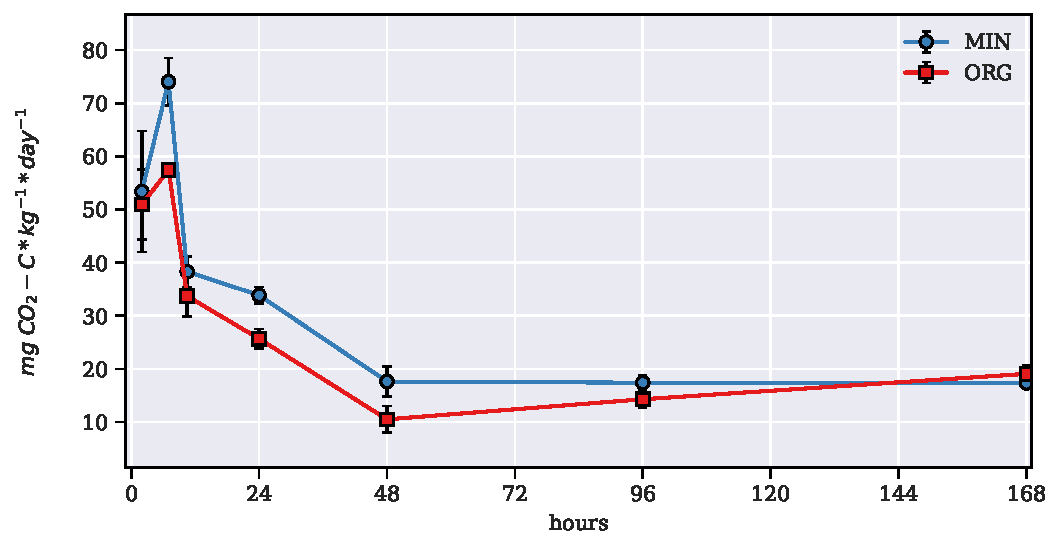
\includegraphics[scale=0.8]{thesis_figures/preliminary/control/Resp.pdf}
  				\caption{$CO_2$ respiration as a function of incubation time in non-amended aoil samples of mineral (MIN) and organic (ORG) plots from the Gilat Fertility Experiment}
  				\label{fig:resp_control_preliminary}
  			\end{figure}

  			\begin{figure}[H]
  				\centering
  				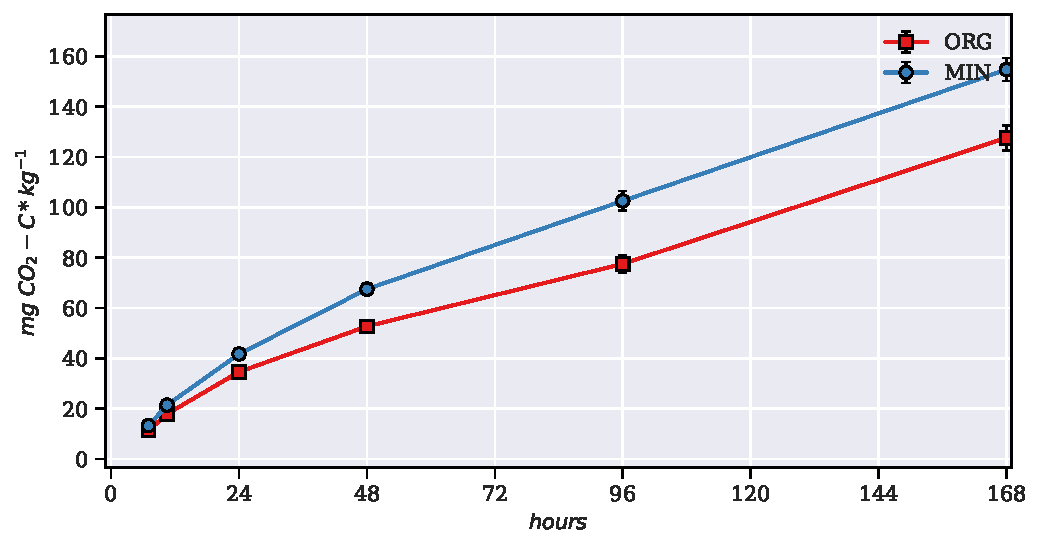
\includegraphics[scale=0.8]{thesis_figures/preliminary/Cum_Resp_CON.pdf}
  				\caption{cumulative $CO_2$ respiration  as a function of incubation time in non-amended samples  of mineral (MIN) and organic (ORG) plots from the Gilat Fertility Experiment}
  				\label{fig:cum_resp_control_preliminary}
  			\end{figure}

            \noindent A slight and evidently statistically insignificant, increase in MBC (Fig \ref{fig:mbc_control_preliminary}) was observed in Min samples after 24 h of incubation, followed by slight decrease in the next 3 days.  In sharp contrast, in Org samples, MBC had seen a substantial increase of $ \tilde{} $100 \genericunit  between 24-48h of incubation. This increase marked a peak of MBC in Org, after which MBC levels declined sharply to reach a value of ~370 \genericunit, same as in Min.

        \begin{figure}[H]
            \centering
            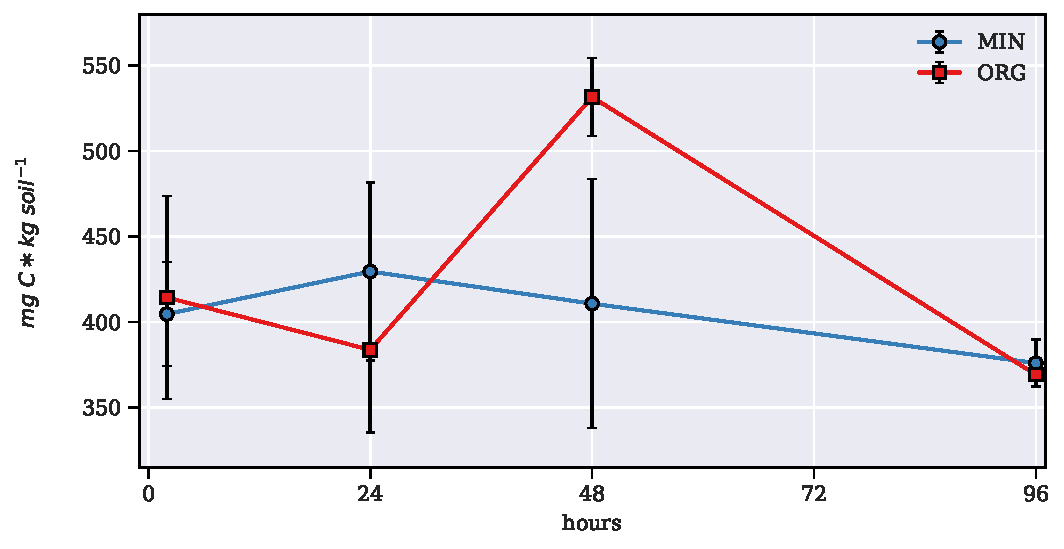
\includegraphics[scale=0.8]{thesis_figures/preliminary/control/MBC.pdf}
            \caption{MBC  as a function of incubation time in non-amended samples  of mineral (MIN) and organic (ORG) plots from the Gilat Fertility Experiment}
            \label{fig:mbc_control_preliminary}
        \end{figure}

        \subsubsection{WEOC}
            WEOC  (Fig \ref{fig:weoc_control_preliminary}) was higher in Org throughout the incubation, with the exception of 48h. Initial levels of WEOC were more than 50$\%$ higher in ORG, with this percentage decreasing to ~30$\%$ after 96 h of incubation. In both LTTs, WEOC was almost without change in the first 24 h, subsequently dropping sharply to reach a relatively similar value of ~20 \genericunit in both LTTs after 48 h of incubation. This sharp decrease was followed by a substantial increase in the next 48 h, finally reaching values  slightly, yet significantly higher than initial values. It is worth noting the opposite trends between \hyperref[fig:mbc_control_main]{MBC} and WEOC, particularly in  Org, whereby  a sharp decrease in WEOC between 24-48 h was accompanied by a similarly sharp increase in MBC, and the same (inverse) contrast was observed in the following 48 h.

            \begin{figure}[H]
            \centering
            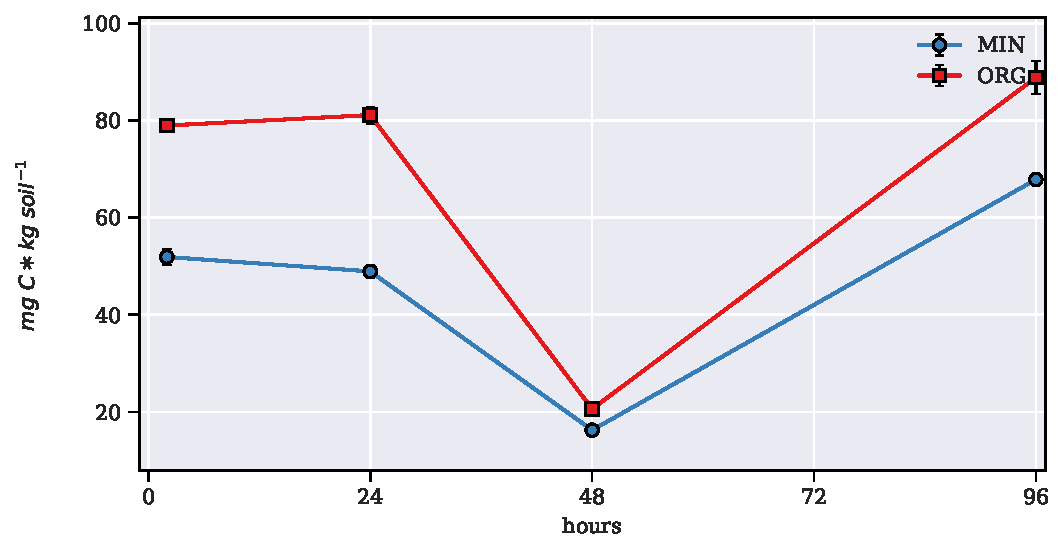
\includegraphics[scale=0.8]{thesis_figures/preliminary/control/WEOC.pdf}
            \caption{WEOC  as a function of incubation time in non-amended samples  of mineral (MIN) and organic (ORG) plots from the Gilat Fertility Experiment}
            \label{fig:weoc_control_preliminary}
             \end{figure}


       	\subsubsection{HWE total Carbon and Carbohydrate-C}

            Org had sustained significantly higher levels of HWEC (Fig \ref{fig:hwec_control_preliminary}) and HWES-C (Fig \ref{fig:hwes-c_control_preliminary}) compared with Min throughout the entire incubation, with Org values 50 and 30$\%$ higher than Min, for HWEC and HWES-C respectivly. HWEC and HWES-C had followed very similar patterns throughout the incubation, in both LTTs, while the dynamics of HWEC fluctuated more sharply in the first 96h in Org but not so much in Min which presented strong concurrence in time dependent changes between HWEC and HWES-C (pearson r = 0.97 for first differences in Min, compared with 0.91 for Org, data not shown). These concurrent dynamics suggest that HWES-C comprised a relatively constant fraction of HWEC in control samples of these two LTT, throughout the incubation period. This fraction, calculated by averaging the ratio of HWES-C-to-HWEC across all sampling events, yielded a mean of 0.33 and 0.29 in Min and Org respectively, with a $\pm$0.01 associated error.

            \begin{figure}[H]
                \centering
                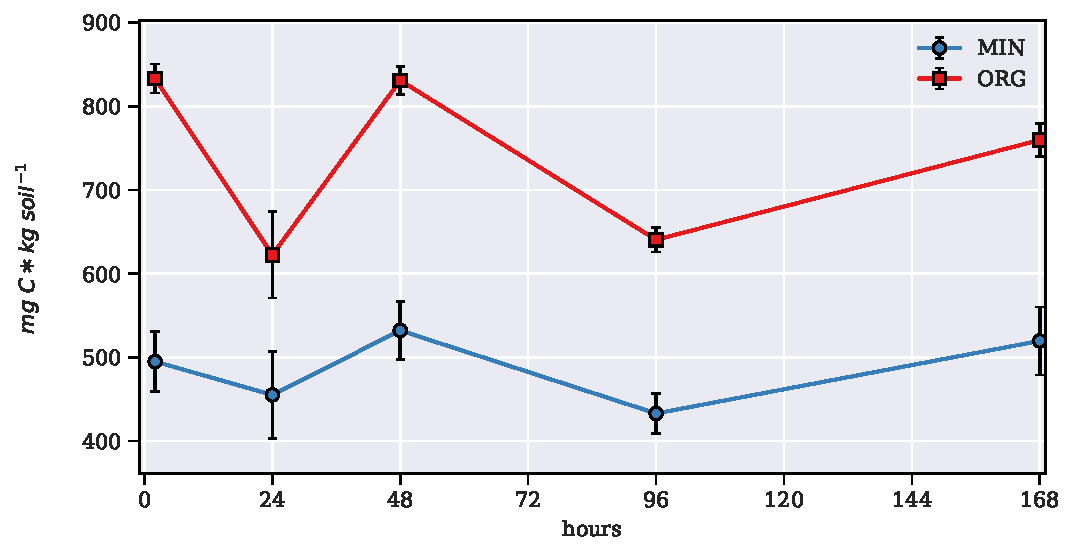
\includegraphics[scale=0.8]{thesis_figures/preliminary/control/HWEC.pdf}
                \caption{HWEC as a function of incubation time in non-amended samples  of mineral (MIN) and organic (ORG) plots from the Gilat Fertility Experiment}
                \label{fig:hwec_control_preliminary}
            \end{figure}

            \begin{figure}[H]
                \centering
                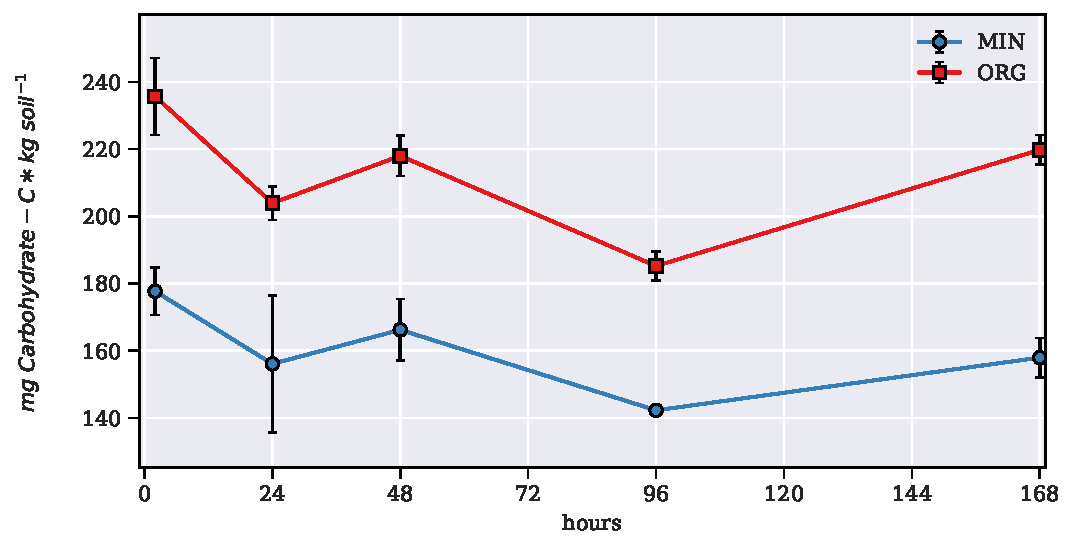
\includegraphics[scale=0.8]{thesis_figures/preliminary/control//HWES-C.pdf}
                \caption{HWES-C  as a function of incubation time in non-amended samples  of mineral (MIN) and organic (ORG) plots from the Gilat Fertility Experiment}
                \label{fig:hwes-c_control_preliminary}
            \end{figure}

        \subsubsection{Ergosterol}
            Min presented a slight, insignificant decrease in Erg during the incubation period, with a mean Erg concentration of ~9 \genericunit, while Org sustained a considerable reduction in Erg concentrations from ~13 \genericunit in the first 24 h to 10.5 \genericunit by the end of the incubation (Fig. \ref{fig:erg_control_preliminary}). the ratio of Erg-to-MBC saw some fluctuations in Org during the incubation, yet these were all statistically insignificant. this ratio remained practically steady in MIN samples (Fig \ref{fig:erg_to_mbc_control_preliminary}). the average Erg-to-MBC ratio in ORG and MIN samples was 3 and 2.36\% respectively.

            \begin{figure}[H]
                \centering
                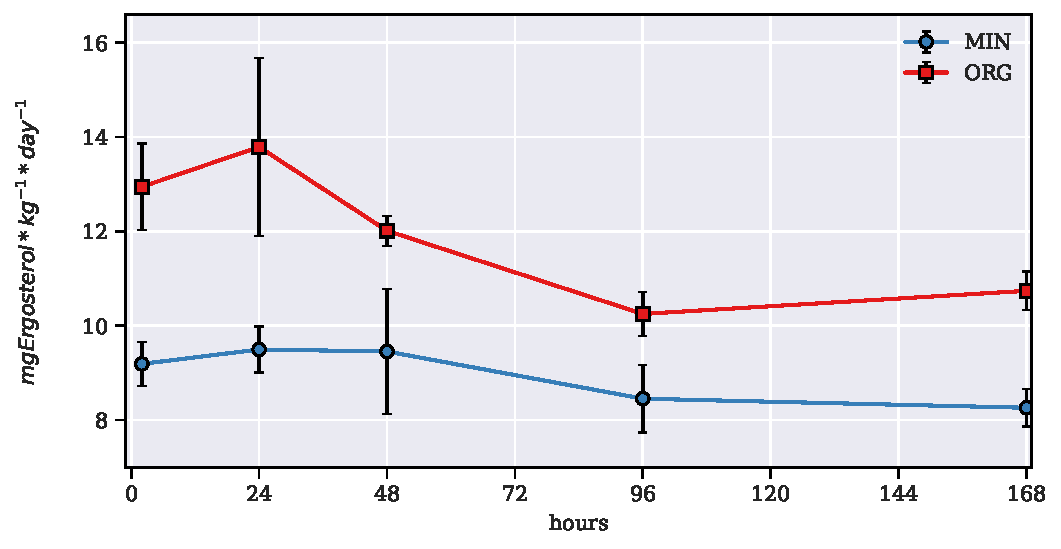
\includegraphics[scale=0.8]{thesis_figures/preliminary/control/Erg.pdf}
                \caption{Ergosterol  as a function of incubation time in non-amended samples  of mineral (MIN) and organic (ORG) plots from the Gilat Fertility Experiment}
                \label{fig:erg_control_preliminary}
            \end{figure}

			\begin{figure}[H]
				\centering
				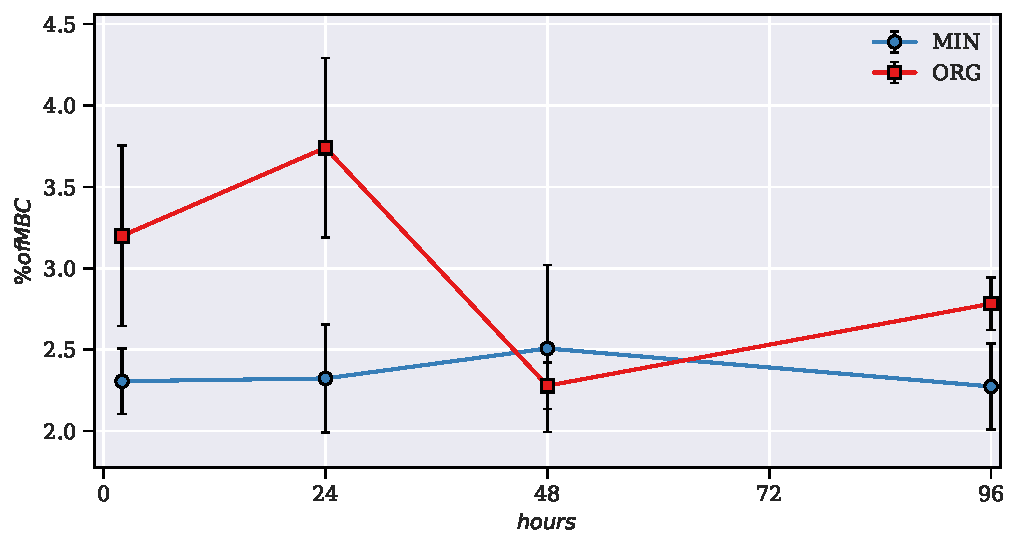
\includegraphics[scale=0.8]{thesis_figures/preliminary/control/Erg-to-MBC_.pdf}
				\caption{Ergosterol-to-MBC  as a function of incubation time in non-amended samples  of mineral (MIN) and organic (ORG) plots from the Gilat Fertility Experiment}
				\label{fig:erg_to_mbc_control_preliminary}
			\end{figure}
%

    \subsection{Dynamics of \gls{som} pools in Straw and KW Compost amended soil}
%todo fix letter symboles overlapping with figure lines in some of the plots


        \subsubsection{Respiration and MBC}
%todo change order of figures to fit the text
%todo cumulative respiration
			Respiration rates and MBC were higher in ORG LTT under both KWC and Str amendment.
            Resp dynamics in the two STTs seem to concur with their respective MBC dynamics (Fig \ref{fig:resp_treated_preliminary}). KWC Resp rates peaked immediately at the onset of the incubation and subsequently decreased rapidly, reaching control normalized values of close to 20 \respunit after 48 hours in both LTTs (Fig \ref{fig:nor_resp_treated_preliminary} B), while STR Resp rates peaked 7 and 10 h after incubation began, in Min and Org respectively (Fig \ref{fig:nor_resp_treated_preliminary} A). Indeed Resp data in KWC is missing for the 7h (as well as 24 h) sampling event, so it is possible that peak rates would have been detected after 7h of incubation. Nonetheless, the substantial difference of more than 150 \genericunit (~75$\%$ ) between the 2h and 10h sampling suggest that, even if this was true, this peak would probably not have been much higher than the observed peak. This intense initial respiration response followed by rapid decline towards control respiration rates, corresponds  to an initial MBC increase in these KWC amended samples. Similarly, a somewhat delayed Resp peak in STR amended samples and relatively high Resp rates sustained throughout the larger part of the incubation, concur with substantial growth in the first 24 h of incubation as well as with the high levels of MBC sustained through the next 72 h in these samples.\\
            	\begin{figure}[H]
            	\centering
            	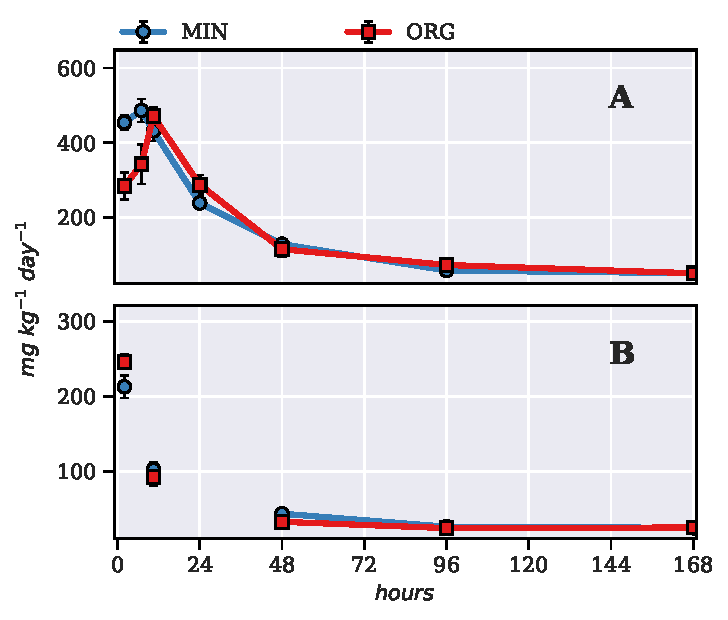
\includegraphics[width=\linewidth]{thesis_figures/preliminary/treated/Resp.pdf}
            	\caption{$CO_2$ as a function of incubation time in in STR $\left(A\right)$ and KWC $\left(B\right)$ amended samples of mineral (MIN) and organic (ORG) plots from the Gilat Fertility Experiment}
            	\label{fig:resp_treated_preliminary}
            \end{figure}

            \begin{figure}[H]
            	\centering
            	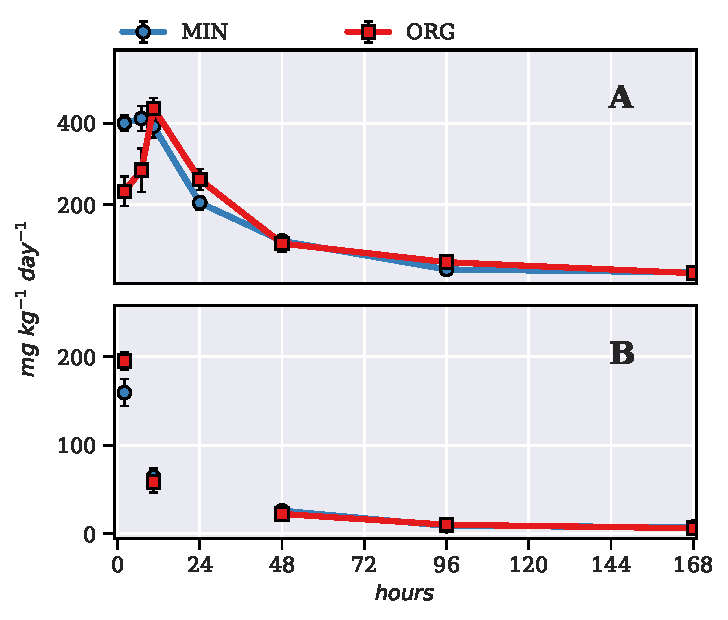
\includegraphics[width=\linewidth]{thesis_figures/preliminary/control_normalized/Resp.pdf}
            	\caption{control normalized $CO_2$  as a function of incubation time in in STR $\left(A\right)$ and KWC $\left(B\right)$ amended samples of mineral (MIN) and organic (ORG) plots from the Gilat Fertility Experiment}
            	\label{fig:nor_resp_treated_preliminary}
            \end{figure}

            \noindent Org had seen an initial increase of 200 and 400 \genericunit MBC over control samples, following the addition of both Str and KWC respectively (Fig \ref{fig:nor_mbc_treated_preliminary}) , while for Min a smaller increase was observed after Str application. Data is missing for Min on the first sampling of KWC  amended samples. Nonetheless, the otherwise parallel MBC trends between the two LTTs ( in KWC amended samples) throughout the rest of the incubation (Fig. \ref{fig:mbc_treated_preliminary}) , suggest a substantial initial increase of ~400 \genericunit over control samples (absolute value of 600 \genericunit MBC at the first sampling)  in Min+STR samples.
            In KWC amended samples, the initial MBC increase (assuming a value of 400 \genericunit Cn\_MBC for Min samples) was followed by a general decrease in both LTTs, suggesting the favorable effect of KWC on MBC,  was short lived, at least in the short-term period recorded in this incubation. Org+KWC had seen a decrease in Cn\_MBC from the initial 382 to 250 \genericunit after 96h of incubation, while Min saw a similar or greater decrease across 4 days of incubation finally reaching a Cn\_MBC value of  110 \genericunit. Moreover, 24 h after the start of the incubation, MBC in Min+KWC samples had decreased by almost 100 \genericunit below the level of corresponding control samples,  suggesting a short-term negative effect of KWC on MBC. In contrast with KWC, STR amendment had initially caused relatively small and little-to-no increases over control samples in Org and Min respectively, while seeing a sharp increase of more than 600 \genericunit in both LTTs after 24 h (~50$\%$ higher than initial increase in KWC amended samples).\\

			\begin{figure}[H]
				\centering
				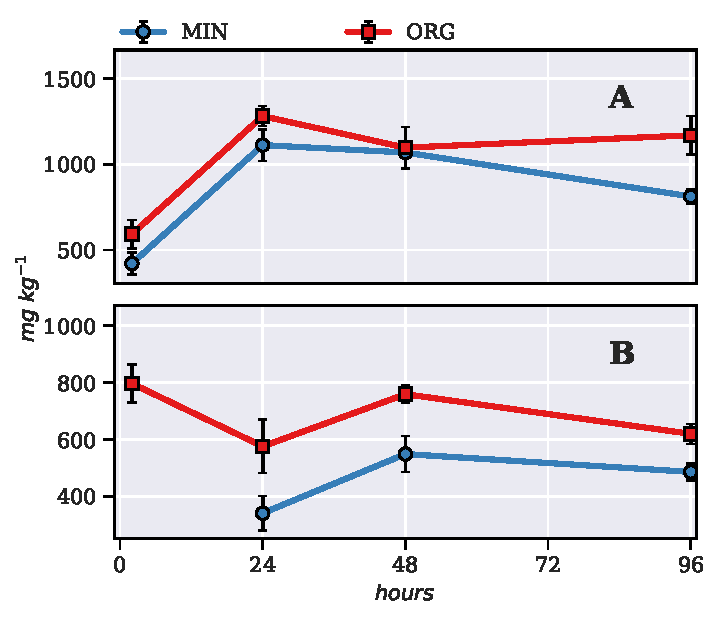
\includegraphics[width=\linewidth]{thesis_figures/preliminary/treated/MBC.pdf}
				\caption{MBC  as a function of incubation time in in STR $\left(A\right)$ and KWC $\left(B\right)$ amended samples of mineral (MIN) and organic (ORG) plots from the Gilat Fertility Experiment}
				\label{fig:mbc_treated_preliminary}
			\end{figure}

			\begin{figure}[H]
				\centering
				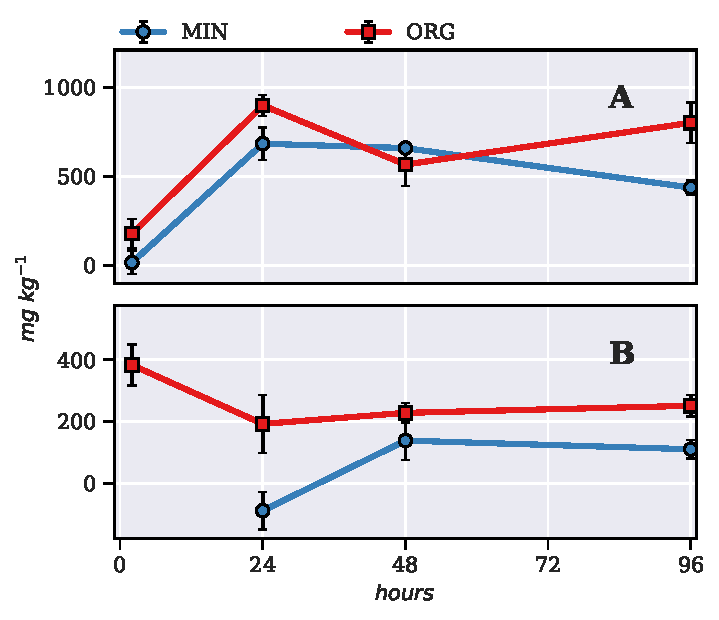
\includegraphics[width=\linewidth]{thesis_figures/preliminary/control_normalized/MBC.pdf}
				\caption{control normalized MBC  as a function of incubation time in in STR $\left(A\right)$ and KWC $\left(B\right)$ amended samples of mineral (MIN) and organic (ORG) plots from the Gilat Fertility Experiment}
				\label{fig:nor_mbc_treated_preliminary}
			\end{figure}
			%thesis_figures/preliminary/treated/Resp.pdf



		\subsubsection{WEOC}
			WEOC dynamics (Fig \ref{fig:weoc_treated_preliminary}) presented a general pattern in all samples, in which the initial increase in WEOC was followed by substantial decline, reaching a minimum level after 48 h and than increasing to varying degrees, depending mostly on STT.  Notably, the decline in WEOC following initial increase was much stronger in STR compared to KWC in the first 24 h, and the overall decrease, in terms of the absolute difference, between the 2h sampling and the 48 h sampling was considerably larger in STR. Additionally, in the last 48 h, KWC samples had increased WEOC levels to values close to initial values, while the corresponding increase in STR was relatively much more limited, with final nor\_WEOC values less than \%30 percent that of initial values. As mentioned earlier for WEOC dynamics of control samples, the WEOC dynamics across the incubation period seem to inversely fit with those of MBC and this observation is made even clearer when considering the variability between the two STTs in this regard. For example, it can be noticed, that in KWC amended samples, MBC levels had seen very little changes in the first 24 h corresponding to the more moderate decrease in WEOC in these samples, compared with the parallel  decrease in STR samples. Similarly, in the last 48 h, a limited increase of WEOC in STR amended samples, corresponds with high levels of MBC while a relatively much larger increase of WEOC in KWC is accompanied by decreasing levels of MBC in these samples.
			\begin{figure}[H]
				\centering
				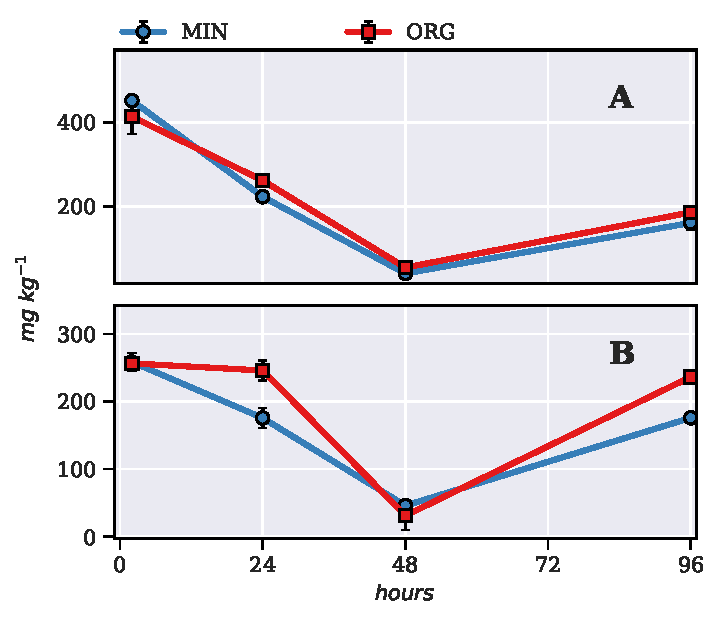
\includegraphics[width=\linewidth]{thesis_figures/preliminary/treated/WEOC.pdf}
				\caption{WEOC  as a function of incubation time in in STR $\left(A\right)$ and KWC $\left(B\right)$ amended samples of mineral (MIN) and organic (ORG) plots from the Gilat Fertility Experiment}
				\label{fig:weoc_treated_preliminary}
			\end{figure}
			similar to microbial biomass and respiration, high Cn\_WEOC (Fig \ref{fig:nor_weoc_treated_preliminary}) values were observed for all treatment combinations in the first sampling. STR amended samples had higher Cn\_WEOC than KWC amended samples, with values  \~{}4 and \~{}8 times higher than control values in Org+STR and Min+STR respectively, compared with \~{}2 and \~{}4 times higher than control in Org+KWC and Min+KWC respectively.


			\begin{figure}[H]
				\centering
				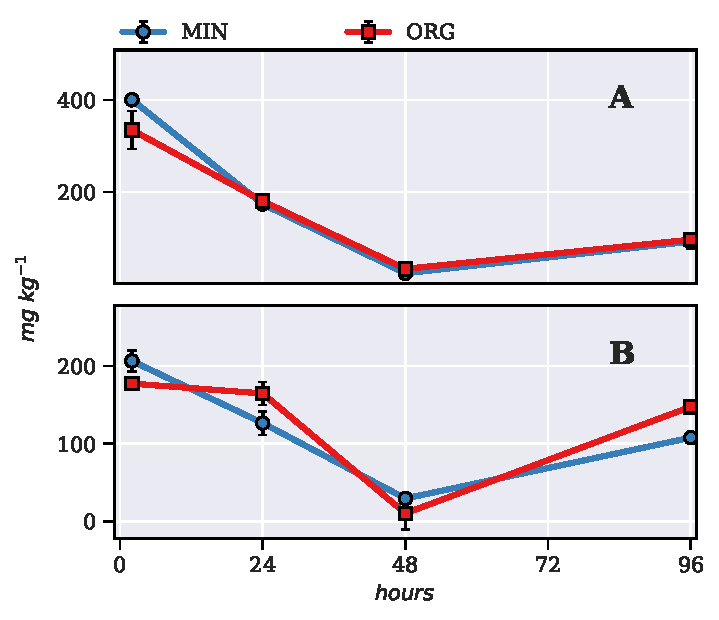
\includegraphics[scale=1]{thesis_figures/preliminary/control_normalized/WEOC.pdf}
				\caption{control normalized WEOC  as a function of incubation time in in STR $\left(A\right)$ and KWC $\left(B\right)$ amended samples of mineral (MIN) and organic (ORG) plots from the Gilat Fertility Experiment}
				\label{fig:nor_weoc_treated_preliminary}
			\end{figure}



		\subsubsection{HWEC and HWES-C}
			In contrast with control samples, where HWEC and HWES levels differed significantly between LTTs during the entire incubation, only few occasions showed significant differences between the two LTTs in STR or KWC amended samples, when results are normalized to control (Fig \ref{fig:nor_hwec_treated_preliminary} and \ref{fig:nor_hwes-c_treated_preliminary}). This may reflect a stronger effect of STTs over the effect of LTTs.
			in Org, KWC and STR had caused relatively small initial increases in Cn\_HWEC and Cn\_HWES-C  , while Min amended samples had seen increases of 67 and 95 \% over control samples in KWC and STR amended samples respectively. In KWC amended samples, both Org and Min samples  had seen a reduction of HWEC (Fig. \ref{fig:hwec_treated_preliminary} B) down to levels below those of control samples after 48 h of incubation and these reductions were followed by an increase back to levels comparable to initial values.
			As observed for control samples, an almost constant ratio of HWES-C-to-HWEC was observed in all STT-LTT combinations, excluding the 48h sampling which saw a sharp increase in this ratio for KWC amended samples (in both LTTs). Although the HWES-C-to-HWEC ratio remained mostly constant, it had slightly increased under KWC and even more so under STR .

			\begin{figure}[H]
				\centering
				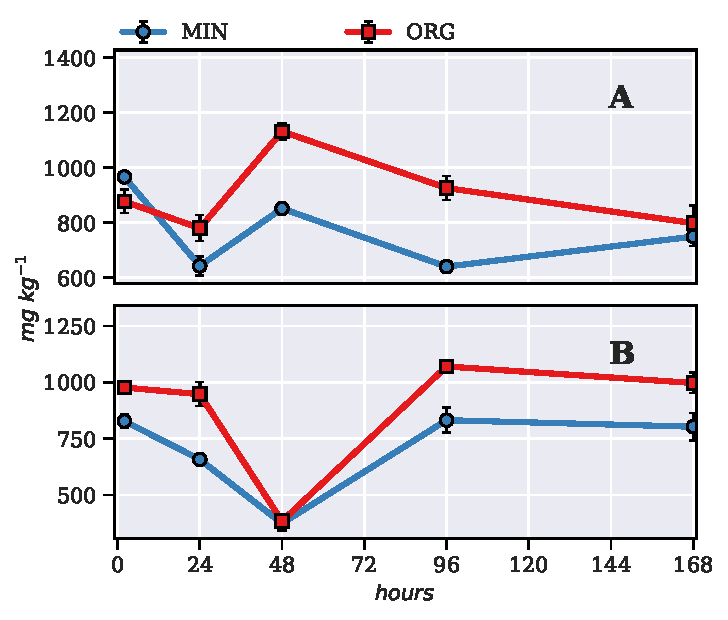
\includegraphics[width=\linewidth]{thesis_figures/preliminary/treated/HWEC.pdf}
				\caption{HWEC  as a function of incubation time in in STR $\left(A\right)$ and KWC $\left(B\right)$ amended samples of mineral (MIN) and organic (ORG) plots from the Gilat Fertility Experiment}
				\label{fig:hwec_treated_preliminary}
			\end{figure}

			\begin{figure}[H]
				\centering
				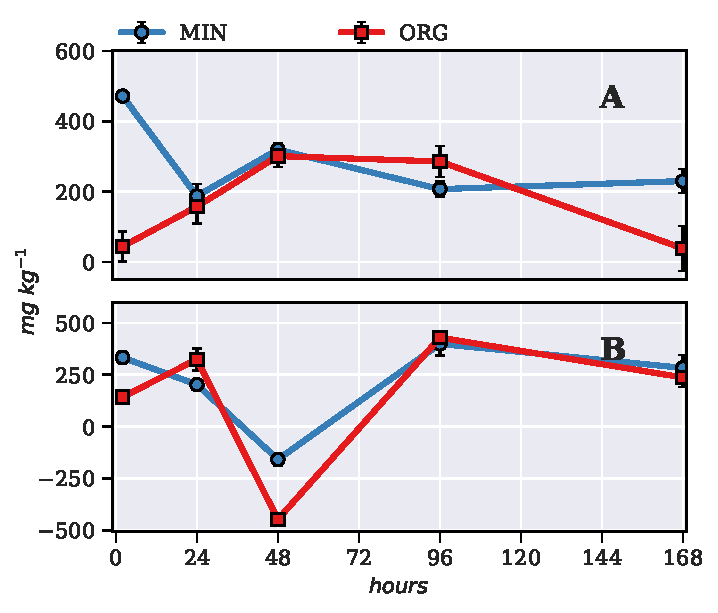
\includegraphics[width=\linewidth]{thesis_figures/preliminary/control_normalized/HWEC.pdf}
				\caption{control normalized HWEC  as a function of incubation time in in STR $\left(A\right)$ and KWC $\left(B\right)$ amended samples of mineral (MIN) and organic (ORG) plots from the Gilat Fertility Experiment}
				\label{fig:nor_hwec_treated_preliminary}
			\end{figure}

			\begin{figure}[H]
				\centering
				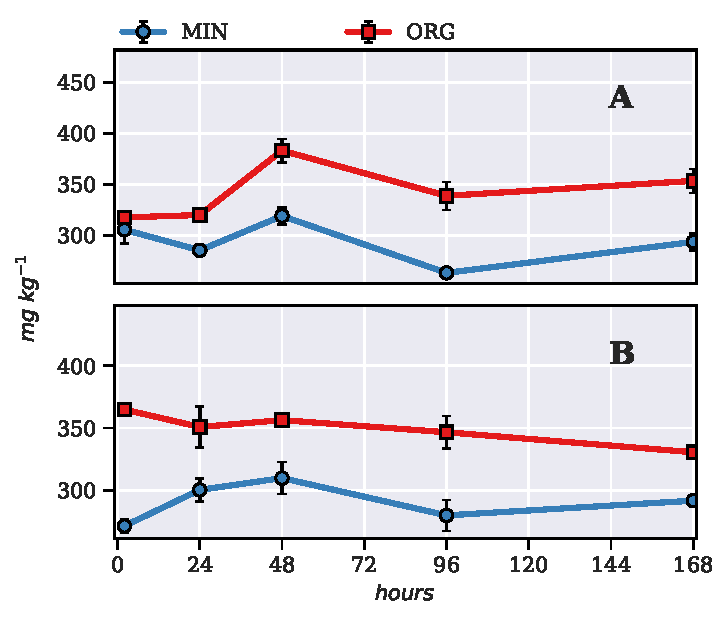
\includegraphics[width=\linewidth]{thesis_figures/preliminary/treated/HWES-C.pdf}
				\caption{HWES-C  as a function of incubation time in in STR $\left(A\right)$ and KWC $\left(B\right)$ amended samples of mineral (MIN) and organic (ORG) plots from the Gilat Fertility Experiment}
				\label{fig:hwes-c_treated_preliminary}
			\end{figure}


			\begin{figure}[H]
				\centering
				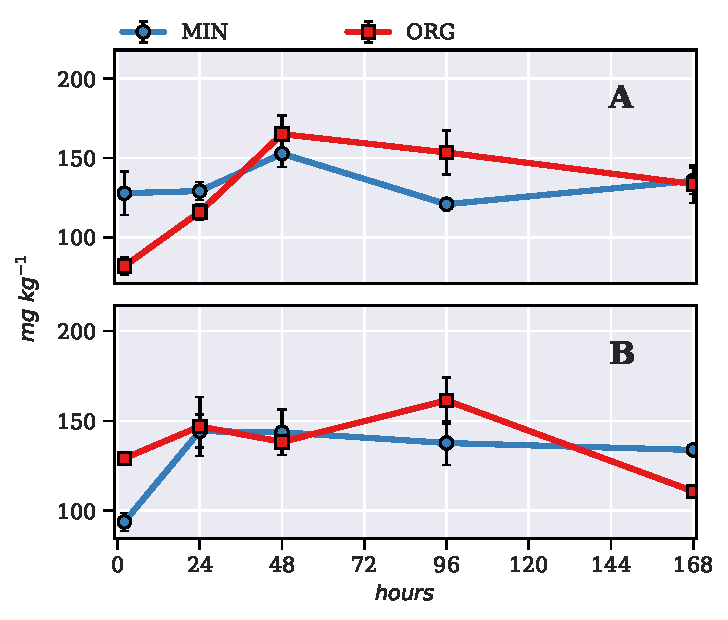
\includegraphics[width=\linewidth]{thesis_figures/preliminary/control_normalized/HWES-C.pdf}
				\caption{control normalized HWES-C  as a function of incubation time in in STR $\left(A\right)$ and KWC $\left(B\right)$ amended samples of mineral (MIN) and organic (ORG) plots from the Gilat Fertility Experiment}
				\label{fig:nor_hwes-c_treated_preliminary}
			\end{figure}

		\subsubsection{Ergosterol}
			In STR amended samples (Fig.\ \ref{fig:erg_treated_preliminary}, A), Ergosterol levels rose sharply during the first 96h in both LTTs and remained high up to the end of the incubation. Contrarily, in KWC amended samples (Fig.\ \ref{fig:hwec_control_preliminary}, B), no significant changes were observed throughout the incubation. in STR amended samples, despite the significant increase in ergosterol concentration, no significant increase in Erg-to-MBC (Fig.\ \ref{fig:erg_to_mbc_treated_preliminary} A) over the corresponding values in the control samples, was observed. this was similarly observed for KWC amended samples (Fig.\ \ref{fig:erg_to_mbc_treated_preliminary} B).

			 \begin{figure}[H]
				\centering
				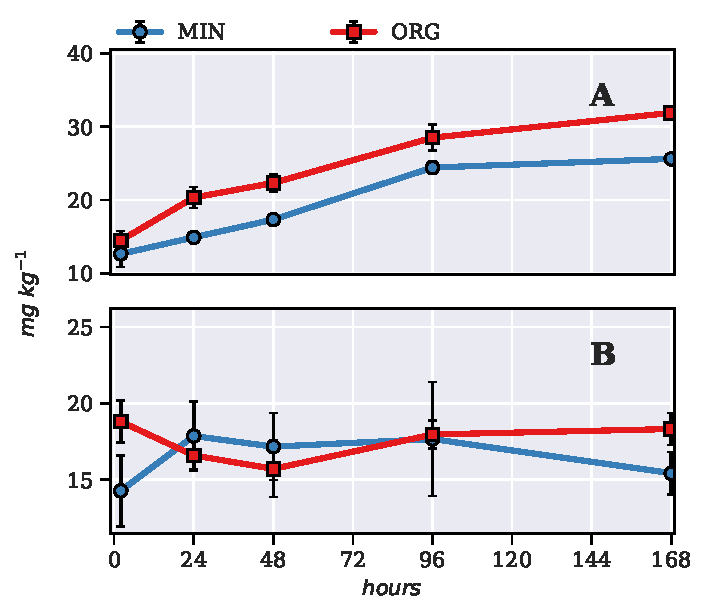
\includegraphics[width=\linewidth]{thesis_figures/preliminary/treated/Erg.pdf}
				\caption{Ergosterol  as a function of incubation time in in STR $\left(A\right)$ and KWC $\left(B\right)$ amended samples of mineral (MIN) and organic (ORG) plots from the Gilat Fertility Experiment}
				\label{fig:erg_treated_preliminary}
			\end{figure}

			\begin{figure}[H]
				\centering
				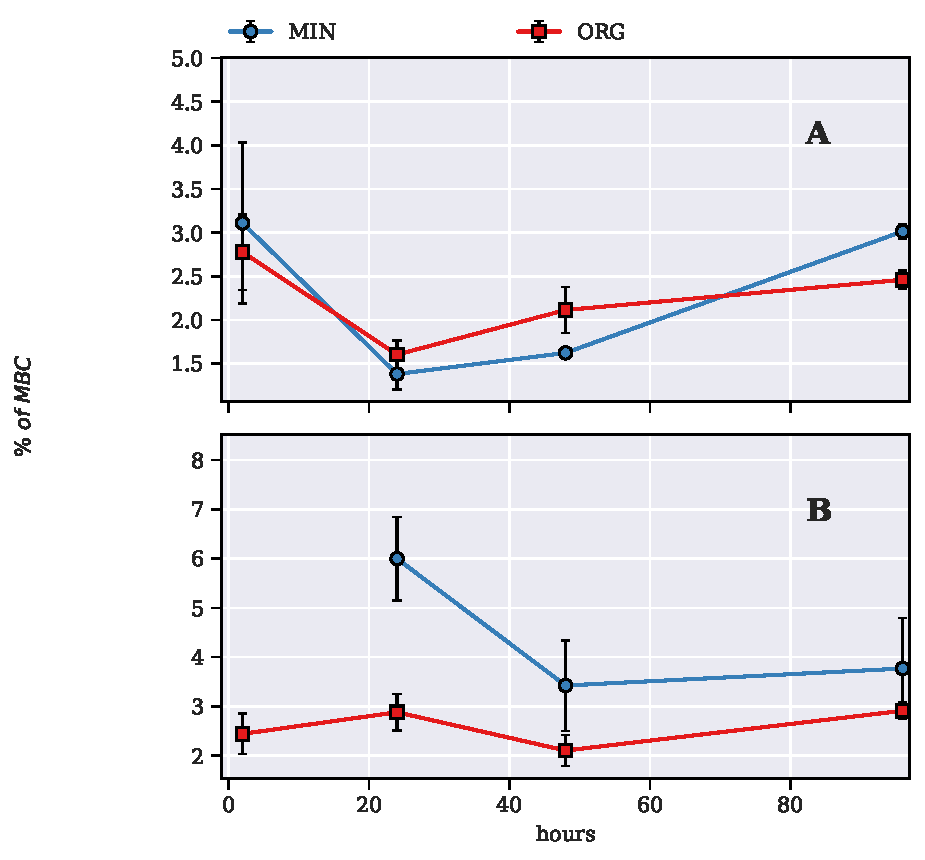
\includegraphics[width=\linewidth]{thesis_figures/preliminary/treated/Erg-to-MBC.pdf}
				\caption{Ergosterol-to-MBC  as a function of incubation time in in STR $\left(A\right)$ and KWC $\left(B\right)$ amended samples of mineral (MIN) and organic (ORG) plots from the Gilat Fertility Experiment}
				\label{fig:erg_to_mbc_treated_preliminary}
			\end{figure}




\section{Incubation with MRE solution}

	This soil incubation experiment was designed as a 28 days incubation which allowed for a more complete evaluation of the effect of long term fertilization treatments on \gls{som} pools (objective \# 1), compared with the one week  preliminary incubation.\\
	In order to examine the effect of long term treatments on short term dynamics of \gls{som} pools (objective \# 2), a highly labile solution of carbonaceous substances was used, simulating a typical root exudate composition. Root exudates are a major source of energy for the soil microbial community. Labile substrates are rapidly processed by micro-organisms and are considerably more likely to be stabilized as minerally associated \gls{om}. This would enable a more detailed examination of the short term \gls{som} dynamics particularly with regards to substrate stabilization. \\
	MRE was applied in three consecutive pulses in order to examine the interaction between substrate load and soil microbial and pyhsical features and how it affected microbial \gls{cue}. \\
	A third LTT was introduced in this incubation in the form of an unmanaged soil, providing a reference point to which \gls{som} changes in the Two other LTT's (ORG and MIN) can be compared.
	In the following section, results for soil parameters that did not include in-week samplings, were presented either as bar plots  or as tables.	weekly MRE/water additions resulted in large in-week fluctuations for the following, frequently sampled for, soil features: MBC, Resp and WEOC (detailed description follows). the remaining soil parameters were only sampled at day 0 and every week end. plotting these data sets as connected lines implies a known variation for the dynamics of between sampling events which is not necessarily the case and therefore a bar plot or table representation was preferred.

	\subsection{\gls{som} properties in non-amended soil samples}

		The first main objective for this work was to establish a reference point  for \gls{som} properties in the three LTTs and evaluate the effect of 5 years of different management histories on the short term dynamics of \gls{som} properties as well as their average baseline values in non-amended samples. As mentioned above, a 4 week incubation was presumed  to better represent the normal fluctuations of \gls{som} pools in a non-amended soil, compared with the results from the shorter, 1 week incubation of non-amended soil which was  included in our preliminary experiment.


		\subsubsection{short-term dynamics}

			the non-amended samples received distilled water as a control for MRE treated samples ( in equivalent volume $=$ 1ml per week).
			each water addition had raised the soil water content by roughly 10$\%$ WHC form 50 to 60$\%$ WHC \pdfcomment[opacity=0.3]{water addition at the begining of each week had raised the water content by about 10\% of Water Holding Capacity}.
			The first water addition was followed by sharp increases in RESP, MBC and  WEOC in all three LTTs (Figures \ref{fig:mbc_control_main}, \ref{fig:resp_control_main} and \ref{fig:weoc_control_main} respectively). Strong pulses of CO2-Respiration were also observed after the 2nd and 3rd water addition. Considerably smaller increases were observed in MBC between days 8-10 and between days 14-15 which seem to have been also related to water additions. These increases following water additions were not observed in WEOC (except for the first water addition). \\
			Regaredless of these pulses, a general trend was observed in the above mentioned parameters, entailing high values during the first part of the incubation (few days to one week depending on the parameter) followed by a decrease and then a steadying of values in later weeks. These similar patterns suggest a connection between microbial growth and activity and the concentrations of WEOC. \\
			Respiration rates rose sharply in the hours following each water addition, peaking after 4h in the 1st and 2nd water additions and after 2h in week 3 (In week 3, no sampling was preformed between 2-12 h after water addition). 4 hours after the first water addition respiration rates were increased by 30$\%$ or more, over the value for 2 h (first sampling), depending on LTT. After A $ \sim $50$\%$ decrease in the next 8 h, rates were mostly  increasing  steadily until the next water addition. The 2nd week saw another, even sharper pulse of respiration, after which respiration rates were constantly decreasing. The 3rd week, similarly saw a sharp increase and then decrease in the first 10 h after water addition and respiration rates subsequently fluctuated within a constant range until the end of that week.\\

			\begin{figure}[H]
				\centering
				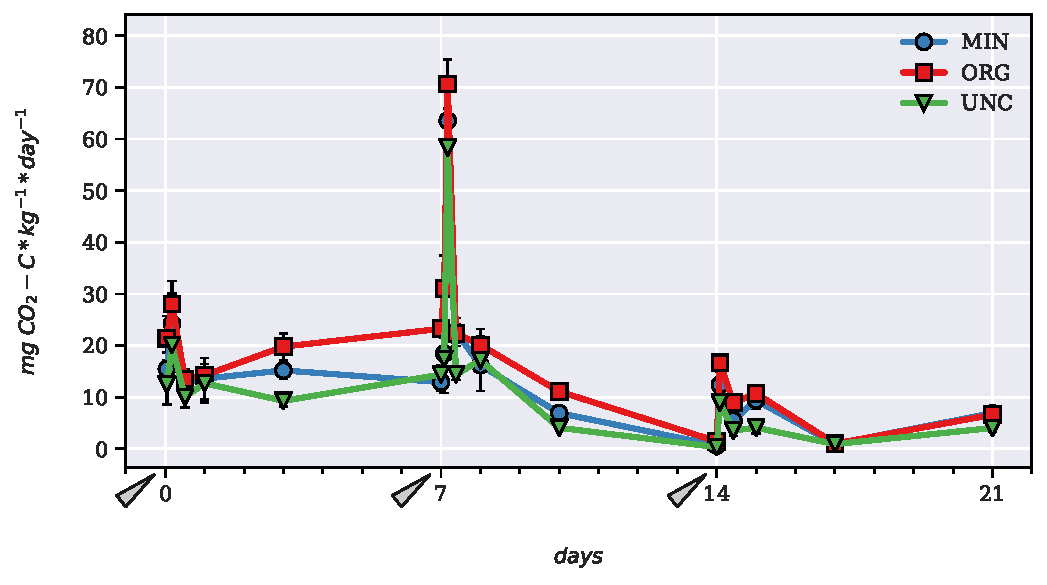
\includegraphics[scale=0.8, width=\linewidth]{thesis_figures/main_incubation/control/Resp.pdf}
				\caption{$CO_2$  as a function of incubation time in non-amendedsamples of mineral (MIN), organic (ORG) and uncultivated (UNC) plots from the Gilat Fertility Experiment}
				\label{fig:resp_control_main}
			\end{figure}
			\noindent MBC had increased by roughly 10 fold in all three LTTs during the first 24 h. Subsequently, MBC levels dropped rapidly, reaching levels comparable to initial values in all three LTTs by the 8th day. from then on, another, slower and more limited in size increase in MBC was observed for all three LTTs, leveling off in the range of 221-464 \genericunit, by the 10th day. A small but significant increase was again observed during the 14th day (immediately after the 3rd water addition) peaking in at 275-564 \genericunit by day 15 and subsequently decreasing slowly to reach values of between ~200-300 \genericunit by the end of the incubation.\\
			\begin{figure}[H]
				\centering
				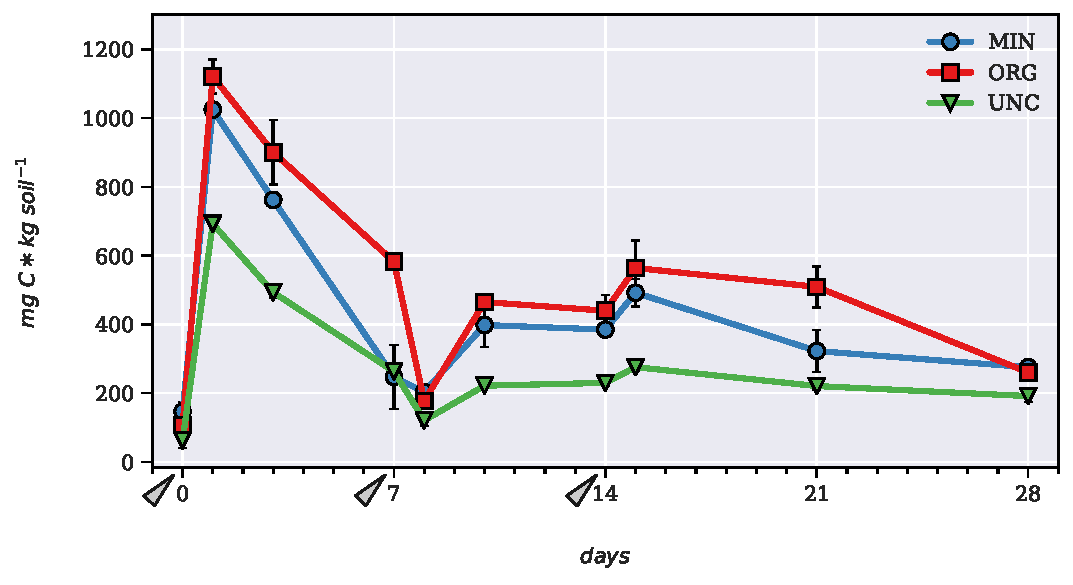
\includegraphics[scale=0.8, width=\linewidth]{thesis_figures/main_incubation/control/MBC.pdf}
				\caption{MBC  as a function of incubation time in non-amendedsamples of mineral (MIN), organic (ORG) and uncultivated (UNC) plots from the Gilat Fertility Experiment}
				\label{fig:mbc_control_main}
			\end{figure}
			\vspace{1cm}
			\noindent Similar to the dynamics of microbial growth and respiration, WEOC  levels had  sharply increased in the first 24 h of incubation (by~300$\%$ in MIN and UNC and ~400$\%$ in ORG), declining considerably during the first half of the 2nd week, and then increasing in the 2nd half and subsequently presenting steady values in the last 2 weeks. In contrast, I did not observe any increases following the 2nd and 3rd water addition, as I did with the dynamics of MBC and particularly those of RESP.  \\


			\begin{figure}[H]
				\centering
				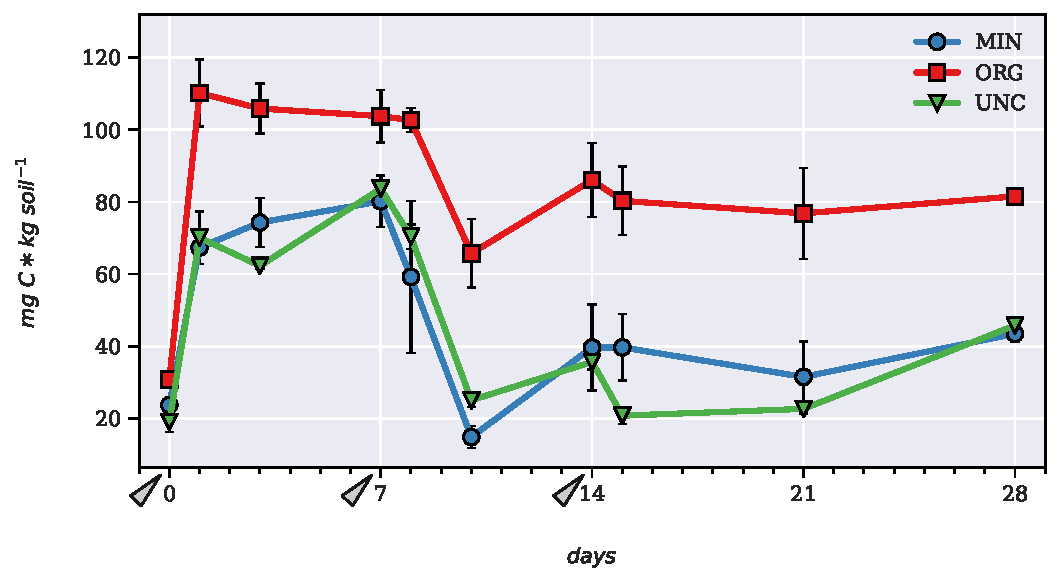
\includegraphics[scale=0.8, width=\linewidth]{thesis_figures/main_incubation/control/WEOC.pdf}
				\caption{WEOC  as a function of incubation time in non-amendedsamples of mineral (MIN), organic (ORG) and uncultivated (UNC) plots from the Gilat Fertility Experiment}
				\label{fig:weoc_control_main}
			\end{figure}

			\noindent HWES (Fig. \ref{fig:hwes_control_main}), in contrast with WEOC, showed only slight changes during the incubation, mostly restricted to the first half of incubation, in which a significant decrease ( particularly in MIN and UNC) and then increase back to levels similar to initial values, was observed. HWES remained practically unchanged during the 2nd half of the incubation. Arguably, HWES samplings were limited to the first and last day of each week and it is possible that more pronounced changes would have been recorded for in-week samplings, as for example, was observed for MBC in the first few days of incubation or for WEOC on day 10. Nonetheless, weekly changes in MBC and WEOC were far more considerable compared with those in HWES, with percent changes in the range of hundreds on the 1st week (MBC and WEOC) and  2nd week (WEOC) (Figs. \ref{fig:mbc_control_main} and \ref{fig:weoc_control_main} for MBC and WEOC respectively). \\
			Interestingly, the period where HWES levels decreased (1st week), correspond to a large extent, with the period of increased MBC, CO2-Resp and WEOC.\\
			Aggregate stability (Table \ref{as_main_control}), measured on days 0, 14 and 28, generally decreased throughout the incubation period, except in ORG in the 2nd half of the incubation.


		\subsubsection{Effect of management history in non-amended samples}

			Overall, the level of \gls{som} parameters observed for control samples throughout the incubation were in the following order, $ ORG  >  MIN  >  UNC $  , However this pattern was somewhat inconsistent in some of the parameters. HWES values (Fig. \ref{fig:hwes_control_main}) for ORG were significantly and substantially higher than for the two other LTTs on every sampling day and WEOC (Fig. \ref{fig:weoc_control_main}) values significantly differentiated ORG from the two other LTTs on 6 out of 10 sampling events. A similar trend is true also for MBC (Fig. \ref{fig:resp_control_main}) concentrations and RESP (Fig. \ref{fig:resp_control_main}) although differences between ORG and MIN soil  are mostly statistically insignificant and the results are generally not as clear. As mentioned above, MIN had mostly higher values than UNC for most parameters throughout the incubation but this was clear only for HWE-S concentrations, where differences between the two soils are statistically significant on every sampling day.
%			\myGreen{emphesize that most parameters distinguished LTTs to \gls{som}e degree}\\

			\begin{figure}[H]
				\centering
				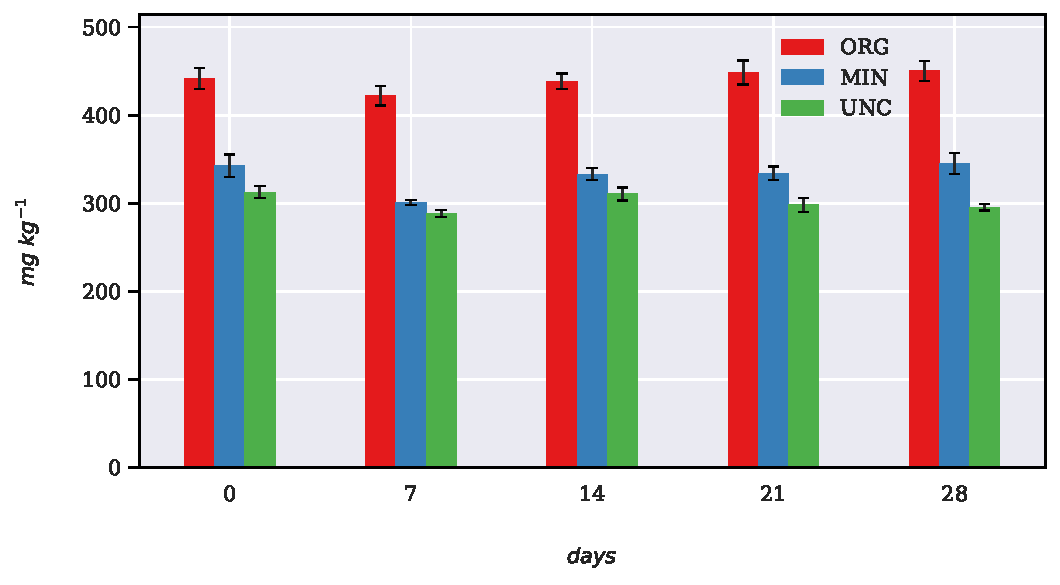
\includegraphics[scale=0.8, width=\linewidth]{thesis_figures/main_incubation/control/HWES.pdf}
				\caption{HWES as a function of incubation time in non-amended samples of mineral (MIN), organic (ORG) and uncultivated (UNC) plots from the Gilat Fertility Experiment}
				\label{fig:hwes_control_main}
			\end{figure}

			\noindent Considerable differences were observed between LTTs in cumulative respiration (Fig \ref{fig:cumulative_control_main} ), in the 2nd and particularly in the 3rd week, with the same order generally observed for other parameters, that is ORG $ > $ MIN $ > $ UNC. Total cumulative respiration after 3 weeks of incubation was 154, 199 and 261 in UNC, MIN and ORG respectively.
				\begin{figure}[H]
				\centering
				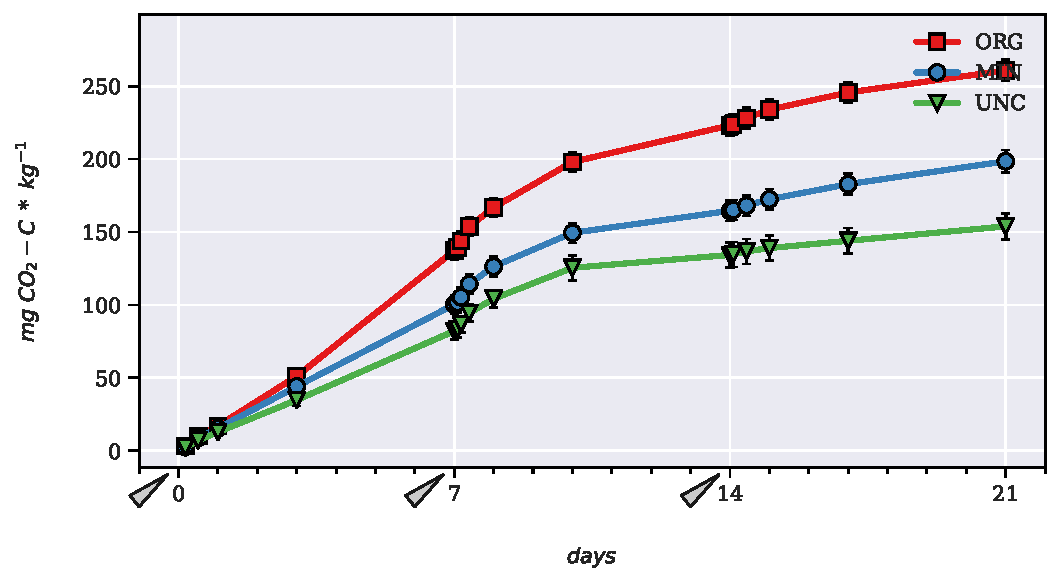
\includegraphics[scale=0.8, width=\linewidth]{thesis_figures/main_incubation/control/Cum_Resp.pdf}
				\caption{Cumulative $CO_2$ respiration  as a function of incubation time in non-amended samples of mineral (MIN), organic (ORG) and uncultivated (UNC) plots from the Gilat Fertility Experiment}
				\label{fig:cumulative_control_main}
				\end{figure}
			\noindent A slight increase in Erg (Fig. \ref{fig:erg_control_main}) was observed for Org and Min during the incubation period while UNC saw an overall slight decrease despite considerable increase in the 1st week . In contrast, Erg as a percent of MBC (Fig. \ref{fig:erg_to_biomass_control_main}) showed a clear reduction in Org and UNC during the 28 days incubation, with most of this decrease occurring in the first half of the incubation. Min samples had seen no significant change in \%Erg of MBC in the course of incubation.
			\begin{figure}[H]
				\centering
				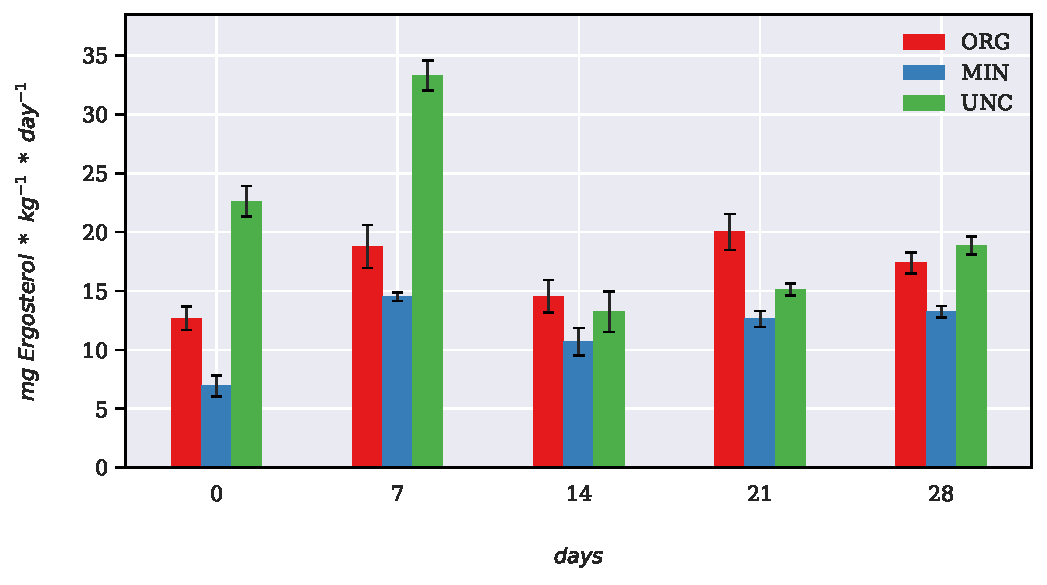
\includegraphics[scale=0.8, width=\linewidth]{thesis_figures/main_incubation/control/Erg.pdf}
				\caption{Ergosterol concentration  as a function of incubation time in non-amended samples of mineral (MIN), organic (ORG) and uncultivated (UNC) plots from the Gilat Fertility Experiment}
				\label{fig:erg_control_main}
			\end{figure}


			\begin{figure}[H]
					\centering
					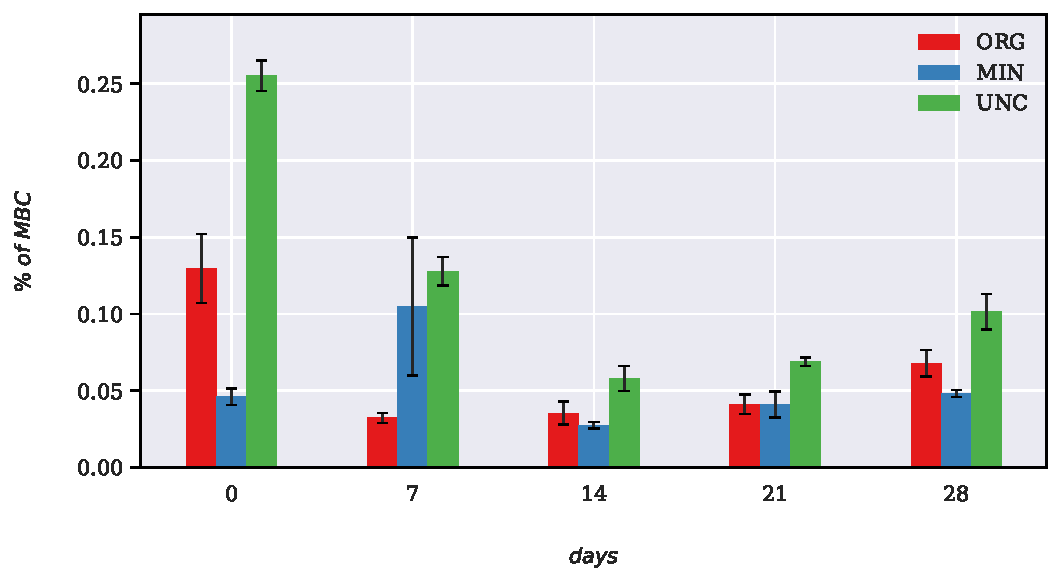
\includegraphics[scale=0.8, width=\linewidth]{thesis_figures/main_incubation/control/Erg-to-MBC.pdf}
					\caption{Ergosterol-to-MBC ratio as a function of incubation time in non-amended samples of mineral (MIN), organic (ORG) and uncultivated (UNC) plots from the Gilat Fertility Experiment}
					\label{fig:erg_to_biomass_control_main}
			\end{figure}
			\noindent as mentioned earlier, the $ \% $WSA (Table \ref{as_main_control}) generally decreased   during the incubation. This was particularly notable in ORG and MIN during the first half of the incubation, with a decrease of more than 5.5\% in both LTTs. A much more limited decrease was observed in UNC during that same period. The total decrease in MIN was roughly double the decrease observed for UNC, while ORG had actually sustained the lowest total decrease in WSA, despite large initial decrease. \\
%			Strong AS decreases in the first half of the incubation in Org and Min, corresponded to strong microbial activity, compared with the second half of the incubation which showed much smaller decreases (and even an increase for Org) and was incidentally also characterized by a more limited microbial growth and seemingly also microbial respiration ( data for the last week not available).
%

			\begin{table}[H]
\centering
\caption{Aggregate Stability, expressed as \%\gls{wsa}, at $ T_0 $, day 14 and day 28 of incubation, in non-amended samples of mineral (MIN), organic (ORG) and uncultivated (UNC) plots from the \gls{gop}}
\label{as_main_control}
\begin{tabular}{llll}
\toprule
\textbf{soil} &            \textbf{MIN} &            \textbf{ORG} &            \textbf{UNC} \\
\textbf{days} &                &                &                \\
\midrule
\textbf{0   } &  19.33 $ \pm $  0.89 &  18.90 $ \pm $  0.89 &  10.42 $ \pm $  0.81 \\
\textbf{14  } &  13.76 $ \pm $  1.63 &  13.31 $ \pm $  1.59 &   9.44 $ \pm $  1.69 \\
\textbf{28  } &  12.85 $ \pm $  0.94 &  17.01 $ \pm $  0.68 &   6.98 $ \pm $  0.35 \\
\bottomrule
\end{tabular}
\end{table}

		\subsubsection{Baseline}
		\label{Baseline}

			Table \ref{baseline_values_of_som_related_properties} shows average values of control samples across day 0 and every week end of the incubation for each LTT (a total of 20 replicates each). Sampling events between week ends were omitted here to eliminate the effect of water additions at the beginning of each week and provide a baseline value that will correspond as accurately as possible to a certain normal level for each parameter-LTT combination.\\
			
\begin{table}[H]
\centering
\caption{Baseline values of SOM pools and associated properties in non-amended soil samples of mineral (MIN), organic (ORG) and uncultivated (UNC) plots from the \gls{gop}}
\label{baseline_values_of_som_related_properties}

\begin{threeparttable}

\begin{tabular}{llllllllll}
\toprule
{} & MBC         &       MBN &      Resp &       HWES &      WEOC &        AS &       Erg &      TOC &      TON \\ 
{} & \scriptsize\genericunit & \scriptsize\genericunit& \scriptsize$ mg\ CO_2$\text{-}$C\ kg^{\text{-}1}\ day^{\text{\text{-}}1}$& \scriptsize\genericunit	& \scriptsize\genericunit & \scriptsize\%WSA& \scriptsize\genericunit& \scriptsize\%weight	& \scriptsize\%weight  \\ \\			
\midrule
ORG &  385.87  a &  49.70  a &  10.43  a &  440.27  a &  75.79  a &  16.69  a &  16.69  b &  1.71  a &  0.15  a \\
MIN &  279.68  a &  50.29  a &   6.81  a &  331.23  b &  43.71  b &  14.95  a &  11.60  c &  1.11  b &  0.09  c \\
UNC &  200.28  b &  32.72  b &   6.79  a &  301.01  c &  41.36  b &   8.81  b &  20.63  a &  1.08  b &  0.10  b \\

\bottomrule
\end{tabular}

\begin{tablenotes}
	\item[*] \scriptsize values represent the mean of replicates sampled throughout the incubation period  (N=20, except for AS, where N=12); Subscript letters represent significance between plots ($ \alpha = 0.05 $). 
\end{tablenotes}

\end{threeparttable}

\end{table}

			the general order of LTTs described above $\left(ORG > MIN > UNC\right)$ for the 28 days dynamics in most soil properties, is similarly maintained when average baseline values are calculated, though significance between LTTs did differ.
			ORG had a significantly higher baseline value in all measured parameters except Erg compared with UNC, while only MBC, AS, and HWES were significantly different between MIN and UNC.
			Differences between ORG and MIN were significant in TOC, WEOC and HWES, while no significant differences were observed in MBC, CO2-Resp and AS between these two LTTs (although all of these parameters were higher in ORG).
			The lack of significance between ORG and MIN in MBC and CO2-Resp rates, probably reflects, to a large extent, the high degree of variability in the data, due to mostly natural and minor technical sources of variability.  Statistical insignificance between ORG and MIN in AS is more likely to reflect actual closer similarity between these two LTTs, at least when compared with UNC. Differences in AS between ORG and MIN were relatively smaller than those in MBC and CO2-Resp, errors were relatively smaller and the difference between UNC and the two other soils was roughly 40\% the maximum AS value (ORG). Thus, it seems that indeed \%WSA, at least for this aggregate size division ( $ >250\mu m$ ), was similar in ORG and MIN.\\
			to summarize, \myRed{our} results suggest that \gls{som} pools in ORG were different from those of the two other LTTs, despite some of these differences not being statistically significant, while MIN and UNC may have been somewhat more similar to each other in terms of \gls{som} properties than each one of them is similar to ORG. Nonetheless, some properties, particularly AS but also MBC and respiration, suggest a considerable distinction between MIN and UNC. \\

%todo format the table with 0 digits


	\subsection{Dynamics of \gls{som} pools in MRE amended soils}

		The results below are presented with regard to the effect of long term soil management on the short term soil reaction to labile organic input (specific objective \# 2).\\



		\subsubsection{Microbial Respiration}

		Similar to MBC (detailed in the following section), CO2-Resp dynamics (Fig \ref{fig:resp_treated_main} ) presented a weekly pulse shortly after each MRE addition, albeit, these pulses were much closer in time to MRE addition than MB growth pulses. In the first two weeks, respiration rates peaked two hours after MRE addition at an average (across LTTs) of 1183 and 623 $mg\ CO2$-$C*kg^{-1}*day^{-1}$ respectively, while the last week saw a considerably smaller peak at 246 $mg\ CO2$-$C*kg^{-1}*day^{-1}$, which was recorded 10 h after MRE addition (no sampling occurred between 2-10 h).
		The high peak respiration rate in the first week, was followed by a general trend of sharp decrease leading to values close to the final value for that week after 3 days of incubation. The second week, unlike the first week, was characterized by a much smaller peak (roughly half the first peak) as well as higher rates in the following days, compared with a similar time period in the first week. These dynamic entailed a considerably more flattened pattern of respiration in the second week. The third pulse was relatively similar to the 2nd pulse (2nd week) in the general pattern, compared with the first pulse, by having a much more limited peak respiration rate and relatively high rates in the next 24 h.\\


		\begin{figure}[H]
			\centering
			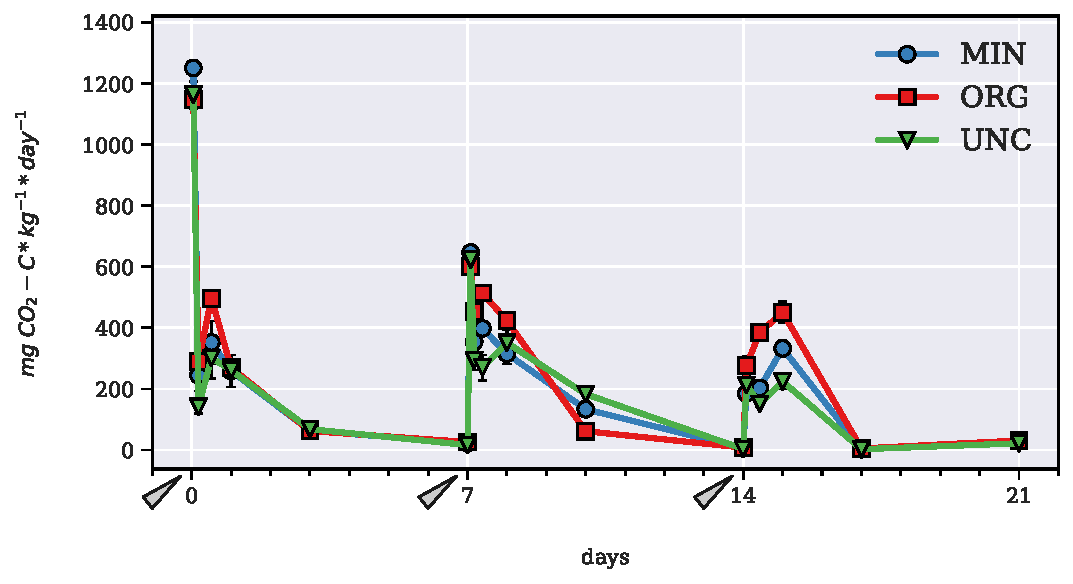
\includegraphics[scale=0.8, width=\linewidth]{thesis_figures/main_incubation/MRE_treated/Resp.pdf}
			\caption{$CO_2$ respiration as a function of incubation time in MRE amended samples of mineral (MIN), organic (ORG) and uncultivated (UNC) plots from the Gilat Fertility Experiment}
			\label{fig:resp_treated_main}
		\end{figure}
		\noindent
		% \myRed{modeling of the general respiration rate dynamics (across all three LTTs) (figure \#), clearly illustrates the changing pattern in respiration between consecutive weeks.
		% 	Using this model for each LTT separately, reveals how these changing patterns between consecutive weeks were differentially  manifested in the different LTTs. This is especially apparent in the second and third weeks. The best fit parameters for each LTT-week with their corresponding stnd error are summarized in table \#}\\
		the average weekly cumulative respiration for all three LTTs (Table \ref{weekly_microbial_growth_and_cumulative_respiration}) rose from 852 \cumrespunit in the 1st week to 1136 \cumrespunit in the 2nd week and than declined again to 659 \cumrespunit in the 3rd week. these weekly values correspond to roughly half or less of the weekly poriton of MRE-C (2200 \genericunit).


		\begin{figure}[H]
			\centering
			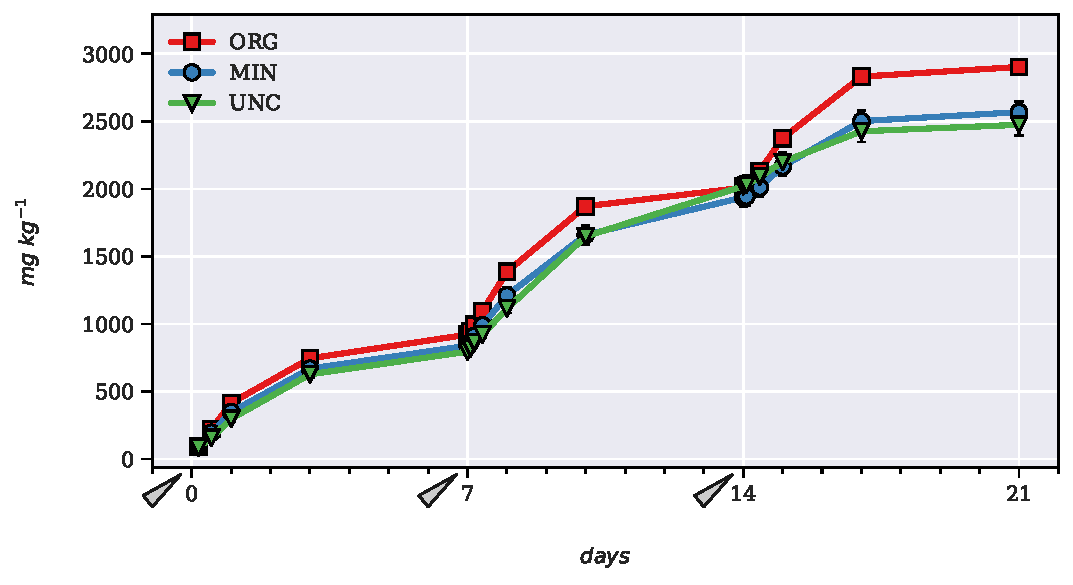
\includegraphics[scale=0.8, width=\linewidth]{thesis_figures/test/Cum_Resp.pdf}
			\caption{cumulative $CO_2$ respiration  as a function of incubation time in MRE amended samples of mineral (MIN), organic (ORG) and uncultivated (UNC) plots from the Gilat Fertility Experiment}
			\label{fig:cum_resp_treated_main}
		\end{figure}

		\subsubsection{Microbial Biomass Carbon}
% todo weekly microbial features table should also include  values as percent of weekly MRE-C.
%todo check significance between the means (across all LTTs) of each week
			The first addition of MRE had a clear and similar effect on MBC in all three soils, as evidenced from the sharp increase of more than 2000 \genericunit that was recorded in all treated soils 24 hours after the addition (figure \ref{fig:mbc_treated_main}). This increase constituted a peak of MBC in the first ­week (as well as the entire incubation) after which MBC dropped by more than a 1000 \genericunit by the beginning of the 3rd day of incubation. This decrease continued in the next few days, reaching average MBC levels of between 500 and 1000 \genericunit in the MRE treated LTTs by the end of the first week. Questionable data collected on the 8th day of incubation (24 h after the 2nd pulse) and missing data from the 17th day of incubation ( 72 h after the 3rd pulse)  make it hard to assert the precise day of peak MBC in the 2nd and 3rd  week. Nonetheless it is highly plausible that a similar trend as in the 1st week of incubation occurred in these two subsequent weeks in all soils, judging from  the more reliable existing MBC data and from RESP data. Assuming that the dynamics of MBC indeed took on the same shape in the 2nd and 3rd week as in the 1st week, it can be seen that every MRE input is followed by a pulse of microbial growth reflected in the sharp increase and then decrease in MBC and RESP.\\



			\begin{figure}[H]
				\centering
				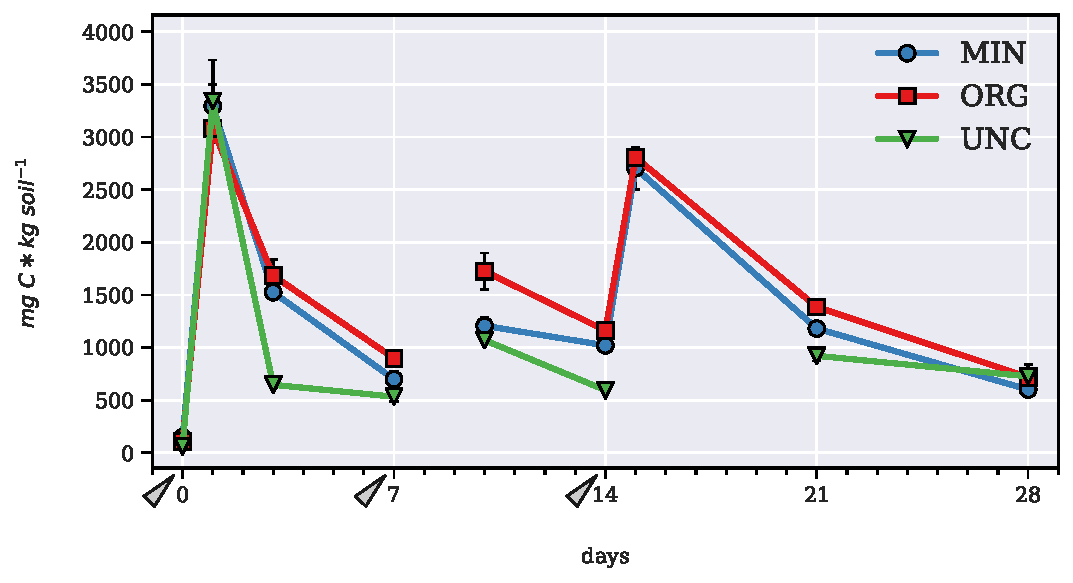
\includegraphics[scale=0.8,width=\linewidth]{thesis_figures/main_incubation/MRE_treated/MBC.pdf}
				\caption{MBC as a function of incubation time in MRE amended samples of mineral (MIN), organic (ORG) and uncultivated (UNC) plots from the Gilat Fertility Experiment}
				\label{fig:mbc_treated_main}
			\end{figure}
			\vspace{1cm}
			\noindent
			the weekly microbial growth in all three LTTs (Table \ref{weekly_microbial_growth_and_cumulative_respiration}) was highest during the 1st week and was then significantly and strongly reduced in the 2nd week,  particularly for ORG and UNC. the 3rd week saw higher growth than in the 2nd week for ORG and UNC but not for MIN. the last week, in which no input was applied, saw substantial negative growth (net decrease in MBC). weekly growth was significantly higher in ORG compared with the two other LTTs in the first week. conversely, ORG saw the strongest negative growth in the last week though this was statistically non-significant. \myRed{Similar trends as described above are observed for net MBC.}\\
			\input{tables/microbial_features_MRE_amended.png}
			similar or very close values of MBC were observed for ORG and MIN soils throughout the incubation with ORG exhibiting slightly higher values on most days (significant on day 8 and 21), while MBC dynamics for UNC diverged, at least to some extent from that of the two other soils with significantly lower values observed on the 3rd and 10th day of incubation ( 3rd day of 1st and 2nd week respectively) as well as on the 14th and 21st day of incubation (end of 2nd and 3rd week respectively). Interestingly, by the end of the incubation, absolute MBC values converged to a similar level of roughly 700 \genericunit in all treated soils. compared with pre-incubation values, this value is equivalent to an increase of  roughly 500-600 \genericunit MBC in the treated soils after 4 weeks of incubation.\\





		\subsubsection{Water Extractable Organic Carbon}
%todo adjust weoc_pct_change plot: vertical lines for sampling dates;
%todo LTT markers;
%todo add extrapolated data point for UNC at day 8 with a dotted line connecting previous and following data point

%todo two seprate plots for WEOC and percent change in cumulative respiration
			Missing WEOC data on the 8th day of incubation prevent a definite description of UNC dynamics in the 2nd week and missing data on the 18th day prevents a detailed description of WEOC dynamics in the the third week for all three LTTs. For day 8, a presumed data point was added based on the trends observed in adjacent weeks.
			The dynamics of WEOC (Fig. \ref{fig:weoc_pct_change_treated_main} ) presented an interesting trend which differed significantly between LTTs. The first MRE addition saw a sharp increase of almost 1000 \genericunit in net WEOC after 24 h in UNC samples whereas only a relatively slight increase of 106 and 33 \genericunit was observed for MIN and ORG respectively. This increase was almost entirely diminished by the 3rd day of incubation in all three LTTs and returned to values very close to the initial values after 7 days. These dynamics were similarly repeated in the 2nd and 3rd weeks, however, WEOC pulses following MRE input increased substantially between subsequent weeks in MIN and UNC. This meant that both the peak of WEOC pulse and its duration (I.e the time period before WEOC returned to baseline level) were increased, with peak WEOC in the second week standing at \~{}500 and \~{}\# \genericunit for MIN and UNC (assumed) respectively, and these values almost doubled in the third week in MIN. In sharp contrast with these two LTTs, WEOC pulses after each MRE addition in ORG were considerably minor, with peak WEOC in the last week amounting to less than 150 \genericunit.
			These contrasting trends between LTTs, inversely correspond with the respective respiration trends in these LTTs. In the second week of incubation, and still more in the 3rd week, lower respiration clearly corresponded with high WEOC pulse as evident from comparing the rate of change in cumulative respiration with pattern of WEOC (Fig \ref{fig:weoc_pct_change_treated_main}).\\
			considering the intensity of these WEOC pulses immediately following MRE additions, and the above mentioned inverse relation with respiration rates, it seems highly likely that the these sharp increases in WEOC largely represent unprocessed substrate.
%
			\begin{figure}[H]
				\centering
			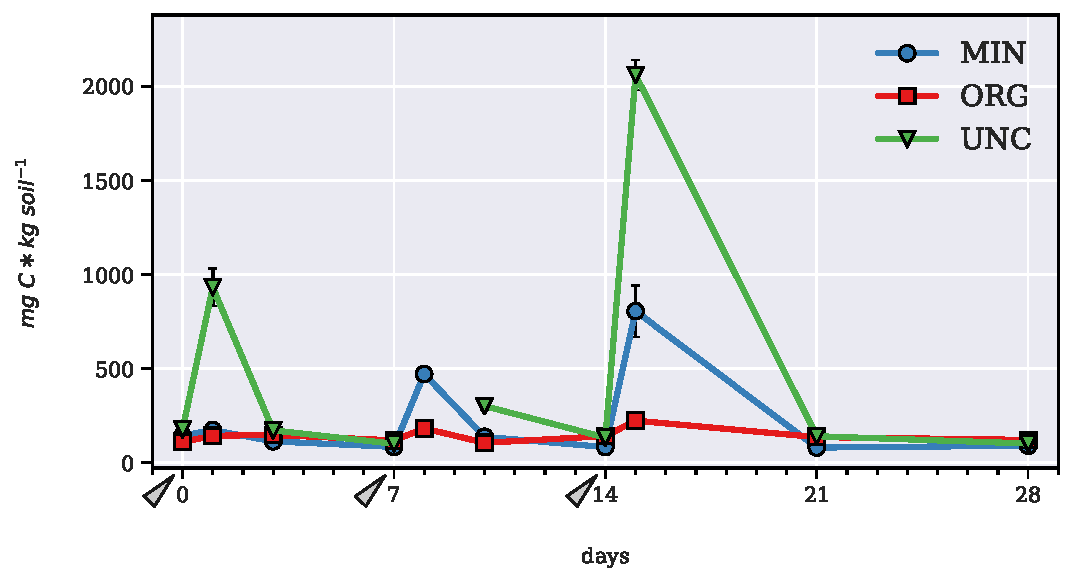
\includegraphics[scale=0.8, width=\linewidth]{thesis_figures/main_incubation/MRE_treated/WEOC.pdf}
				\caption{WEOC as a function of incubation time in MRE amended samples of mineral (MIN), organic (ORG) and uncultivated (UNC) plots from the Gilat Fertility Experiment}
				\label{fig:weoc_treated_main}
			\end{figure}

			\begin{figure}[H]
				\centering
				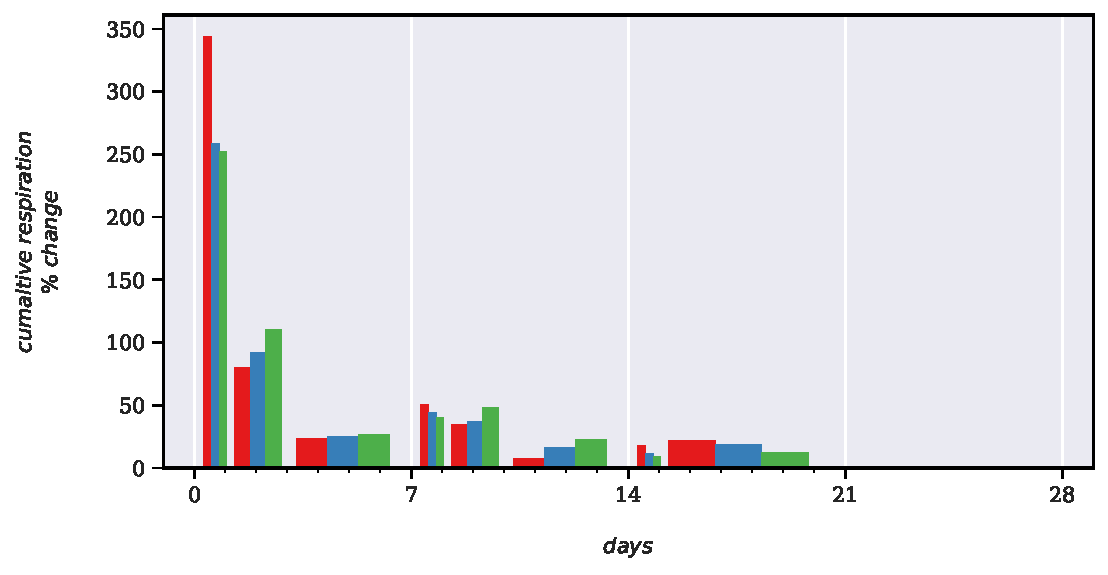
\includegraphics[scale=0.8, width=\linewidth]{thesis_figures/main_incubation/MRE_treated/weoc_pct_change.pdf}
				\caption{Percent change in cumulative respiration for every sampling interval (corresponding to WEOC sampling intervals); Although data is only available for first 3 weeks, plot includes last week of incubation to allow simple comparison with WEOC dynamics.}
				\label{fig:weoc_pct_change_treated_main}
			\end{figure}

		\subsubsection{Hot water extractable sugars}
		%todo add net HWES plot
			Throughout the incubation period, ORG maintained highest absolute values of HWES whereas on the final sampling date a comparable level of HWES (roughly 500 \genericunit) was observed for all treated soils (Fig \ref{fig:hwes_treated_main}). ORG  had the highest HWES at the end of the incubation but this result was highly insignificant. UNC and MIN presented similar absolute values of HWES throughout the incubation. This probably reflects, at least to a certain degree their respective \gls{som} stocks compared with ORG as HWES are often correlated with SOC.
			When these results are normalized to the control value (Fig. \ref{fig:hwes_control_normalized_treated_main}), a different prospect of the HWES dynamics emerges, whereby during the first two weeks the three LTTs maintained similar values while the last two weeks saw a clear divergence between UNC and the two other LTTs. The first week saw an increase of 100 \genericunit or less over control values in all three LTTs and the 2nd week saw a similar increase in all three LTTs. In contrast, during the third week, UNC saw a considerable increase of \~{}50 \genericunit while insignificant changes were observed for ORG and MIN. the last week saw a very similar reduction of \~{}50 \genericunit in MIN and UNC and roughly double that reduction in ORG. significant difference was observed between UNC and the two cultivated LTTs on the the last sampling event but not between ORG and MIN.

			\begin{figure}[H]
				\centering
				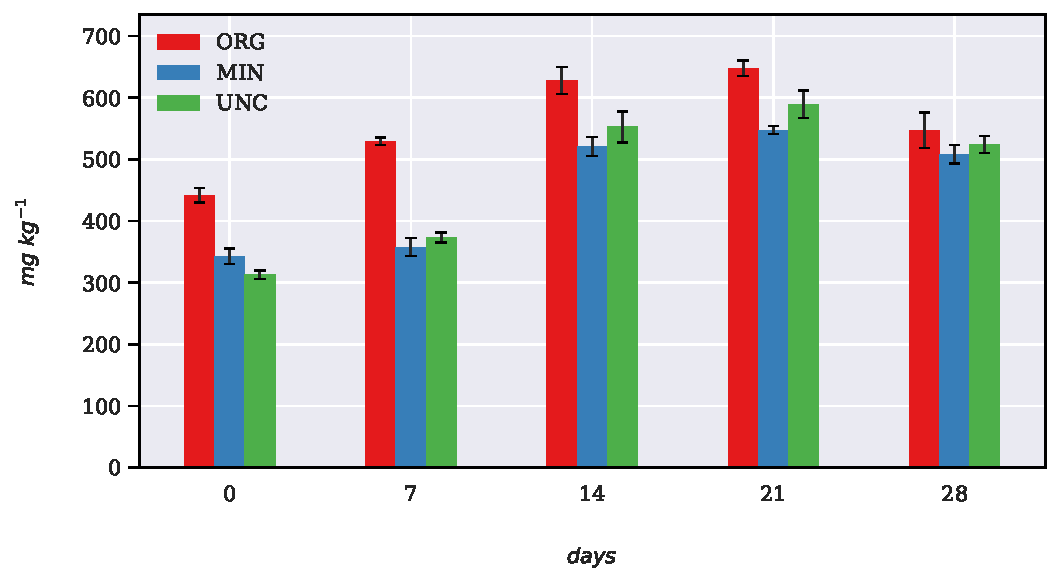
\includegraphics[scale=0.8, width=\linewidth]{thesis_figures/main_incubation/MRE_treated/HWES.pdf}
				\caption{ \footnotesize	HWES as a function of incubation time in MRE amended samples of mineral (MIN), organic (ORG) and uncultivated (UNC) plots from the Gilat Fertility Experiment}
				\label{fig:hwes_treated_main}
			\end{figure}

			\begin{figure}[H]
				\centering
				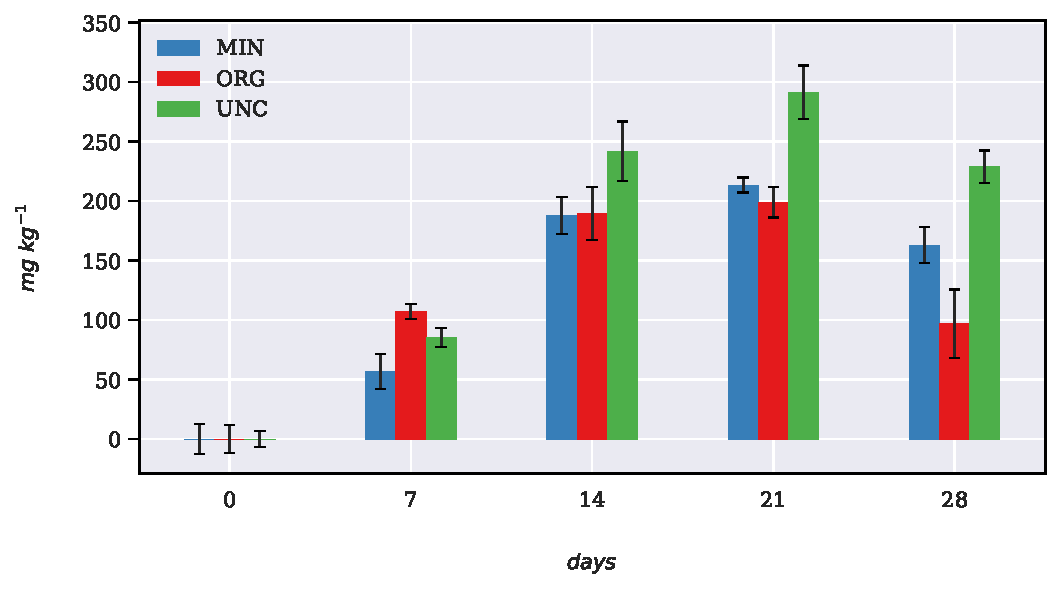
\includegraphics[scale=0.8, width=\linewidth]{thesis_figures/main_incubation/control_normalized/HWES.pdf}
				\caption{HWES normalized to control values as a function of incubation time in MRE amended samples of mineral (MIN), organic (ORG) and uncultivated (UNC) plots from the Gilat Fertility Experiment}
				\label{fig:hwes_control_normalized_treated_main}
			\end{figure}

		\subsubsection{Microbial biomass nitrogen and C/N ratio}
			MBN values in MRE treated soils (figure \ref{fig:mbn_treated_main}) ranged between roughly 10 to 150 \genericunit. MBN dynamics for ORG and MIN were similar in general trend. A sharp increase of roughly  7 fold was observed in first two weeks for MIN and ORG soil. In the 3rd week, increases were very small and the 4th week resulted in a slight decrease for MIN and a much larger decrease for ORG bringing the two LTT’ to a similar value of between 80-90 \genericunit.no apparent increase in MBN was observed For UNC in the 1st week. In the 2nd week an increase comparable to that of the two other soils was measured and from then on MBN levels stayed relatively steady, reaching a final value of 60 \genericunit.\\
%			\myGreen{explain steady MBN in the 1st week for UNC while MBC increased showing extremely high C/N ratio}\\
			Microbial C-to-N ratio ranged from roughly 6 to 11 for the three soils,  throughout the incubation (fig \ref{fig:c_n_ratio_treated_main}), with the highest significant value observed for UNC (11.03) after 3 weeks of incubation.
			An increase in microbial C-to-N ratio over initial value was visible on day 7, 14 and 21 for UNC and ORG while values for MIN stayed relatively steady, with only minor increases in these sampling days. The last week of incubation resulted in a decrease in normalized C-to-N ratio,  especially for UNC and ORG. almost completely undoing the prior increases for MIN, while values for UNC remained relatively high ( differences between MIN and UNC insignificant).

			\begin{figure}[H]
				\centering
				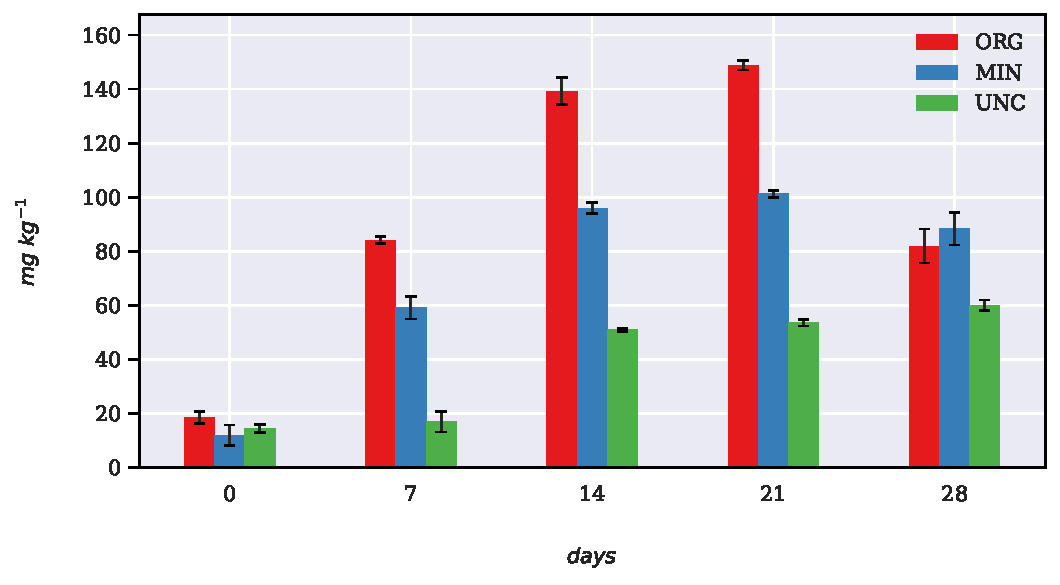
\includegraphics[scale=0.8, width=\linewidth]{thesis_figures/main_incubation/MRE_treated/MBN.pdf}
				\caption{MBN  as a function of incubation time in MRE amended samples of mineral (MIN), organic (ORG) and uncultivated (UNC) plots from the Gilat Fertility Experiment}
				\label{fig:mbn_treated_main}
			\end{figure}

			\begin{figure}[H]
				\centering
				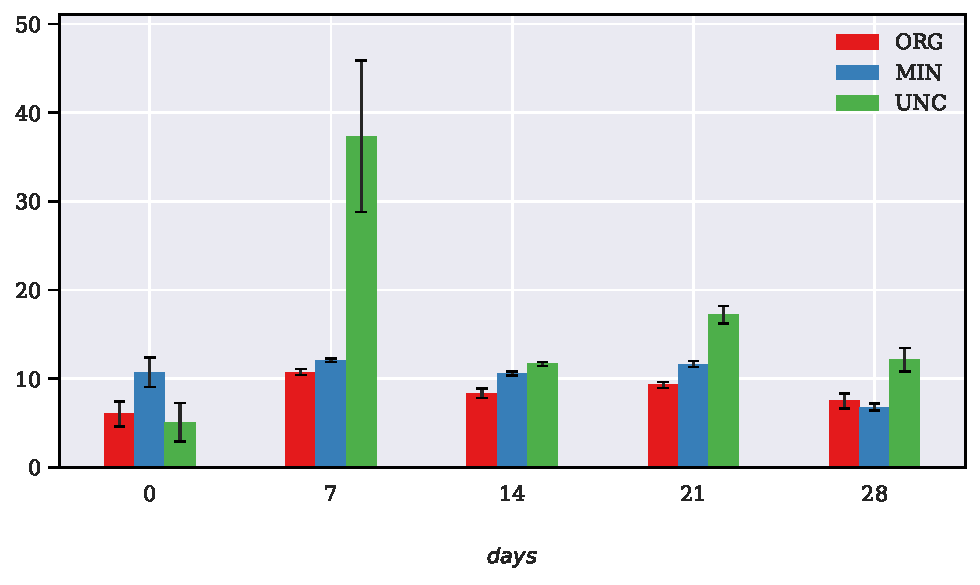
\includegraphics[scale=0.8, width=\linewidth]{thesis_figures/main_incubation/MRE_treated/C_N_ratio.pdf}
				\caption{C/N ratio  as a function of incubation time in MRE amended samples of mineral (MIN), organic (ORG) and uncultivated (UNC) plots from the Gilat Fertility Experiment}
				\label{fig:c_n_ratio_treated_main}
			\end{figure}





		\subsubsection{Ergosterol-to-microbial biomass (ERG-to-MBC)}

			The ratio of ERG-to-MBC dropped sharply in the first week of incubation in both ORG and UNC, with a more moderate decrease in 	MIN, and reached a similar value of  roughly 0.05\% in all three soils. From then onwards, ERG-to-MBC remained relatively steady, with a slight decrease and then increase in the fertilized soils, during the $2^{nd}$ and $ 4^{th} $ weeks respectively. By the end of 4 weeks of incubation,  ERG-to-MBC values were practically identical at \~{}0.03\%, again indicative of the strong effect of MRE treatment compared with the effect of long-term management treatments.

			\begin{figure}[H]

				\centering
				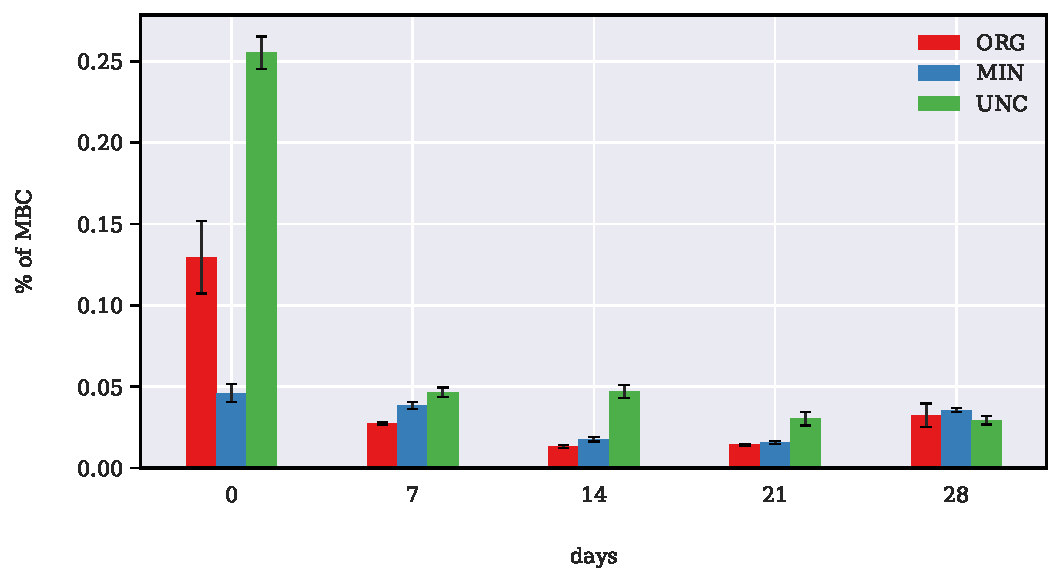
\includegraphics[scale=0.8, width=\linewidth]{thesis_figures/main_incubation/MRE_treated/Erg-to-MBC.pdf}
				\caption{Ergosterol as a function of incubation time in MRE amended samples of mineral (MIN), organic (ORG) and uncultivated (UNC) plots from the Gilat Fertility Experiment}
				\label{fig:erg_treated_main}
			\end{figure}

		\vspace{5cm}

		\subsubsection{Carbon Use Efficiency}
		The weekly trend in \gls{cue} (Table \ref{cue_treated_main}) seemed to differ between the cultivated LTTs and the non-cultivated LTT. Both cultivated LTTs presented a sharp decrease of \~{}50\% in \gls{cue} between the 1st and 2nd week with values staying practically the same between the 2nd and 3rd week. by contrast UNC saw an even more pronounced decrease in \gls{cue} between the 1st and 2nd week (about 10 fold) while the 3rd week actually saw a sharp increase compared with the 2nd week, with a \gls{cue} similar to that observed in the 1st week.


		\begin{table}[H]
\centering
\caption{weekly Carbon Use Efficiency during first three weeks of the incubation, in MRE amended samples of mineral (MIN), organic (ORG) and uncultivated (UNC) plots from the \gls{gop}}
\label{cue_treated_main}

\begin{threeparttable}


\begin{tabular}{llll}
\toprule
\textbf{soil} &           MIN &           ORG &           UNC \\
\textbf{week} &               &               &               \\
\midrule
\textbf{1   } &  0.40 $ \pm $  0.06 &  0.46 $ \pm $  0.02 &  0.37 $ \pm $  0.04 \\
\textbf{2   } &  0.23 $ \pm $  0.06 &  0.20 $ \pm $  0.03 &  0.05 $ \pm $  0.04 \\
\textbf{3   } &  0.20 $ \pm $  0.07 &  0.20 $ \pm $  0.05 &  0.42 $ \pm $  0.07 \\
\bottomrule
\end{tabular}

\begin{tablenotes}
	\item[*] \scriptsize values represent a mean of 4 replicates along with standard error;
\end{tablenotes}

\end{threeparttable}

\end{table}



		\subsubsection{Aggregate stability}

		Aggregate stability was measured three times during the incubation, at $ T_0 $, day 14 and day 28. The percentage of stable aggregate was increased by more than 20\% in the course of the incubation in all three soils (Table \ref{as_main_treated}). For ORG and UNC, \~{}80\% of the stable aggregates formed during the incubation period were formed in the first half of the incubation, while MIN samples presented almost similar increases in percentage of stable aggregates in the second half as in the first half of incubation. UNC had the lowest value of \%WSA in all three samplings.\\

		\begin{table}[H]
\centering
\caption{Aggregate Stability, expressed as \%\gls{wsa}, at $ T_0 $, day 14 and day 28 of incubation, in MRE amended samples of mineral (MIN), organic (ORG) and uncultivated (UNC) plots from the \gls{gop}}
\label{as_main_treated}
\begin{threeparttable}
\begin{tabular}{llll}
\toprule
\textbf{soil} &            MIN &            ORG &            UNC \\
\textbf{days} &                &                &                \\
\midrule
\textbf{0   } &  19.33 $ \pm $  0.89 &  18.90 $ \pm $  0.89 &  10.42 $ \pm $  0.81 \\
\textbf{14  } &  31.87 $ \pm $  2.72 &  36.71 $ \pm $  1.69 &  28.30 $ \pm $  2.45 \\
\textbf{28  } &  45.47 $ \pm $  1.92 &  41.57 $ \pm $  1.49 &  34.04 $ \pm $  1.81 \\
\bottomrule
\end{tabular}

\begin{tablenotes}
	\item[*] \scriptsize values represent a mean of 4 replicates along with standard error;
\end{tablenotes}

\end{threeparttable}
\end{table}



%		\begin{figure}[H]
%			\centering
%			\includegraphics[scale=0.8]{thesis_figures/main_incubation/MRE_treated/\gls{cue}.pdf}
%			\caption{\gls{cue} in MRE amended samples}
%			\label{fig:cue_treated_main}
%		\end{figure}
%
